%--------------------
% SETARI
%--------------------
\documentclass[
	12pt, % mărimea fontului
	twoside % pentru ambele părti ale paginii
]{report}
\usepackage[english, romanian]{babel} % text în engleză sau în română
\usepackage[utf8]{inputenc} % utf-8

%\renewcommand{\baselinestretch}{1.5}
\usepackage{setspace} % spațiul dintre rânduri
\setstretch{1.5} % spațiul dintre rânduri

\usepackage{mathptmx} % times new roman font

\usepackage{geometry}
\geometry{
	paper=a4paper, % stilul documentului
	inner=2.5cm, % marginea interioară
	outer=3.8cm, % marginea exeterioară
	bindingoffset=.5cm, % binding offset
	top=3.1cm, % marginea de sus
	bottom=3.1cm, % marginea de jos
	portrait
}

\usepackage{amsmath} % math symbols

\usepackage{titlesec}
\titleformat{\chapter}[display]
{\normalfont\huge\bfseries}{\chaptertitlename\ \thechapter}{20pt}{\Huge}
\titleformat{\section}
{\normalfont\Large\bfseries}{\thesection}{1em}{}
\titleformat{\subsection}
{\normalfont\large\bfseries}{\thesubsection}{1em}{}
\titleformat{\subsubsection}
{\normalfont\normalsize\bfseries}{\thesubsubsection}{1em}{}
\titleformat{\paragraph}[runin]
{\normalfont\normalsize\bfseries}{\theparagraph}{1em}{}
\titleformat{\subparagraph}[runin]
{\normalfont\normalsize\bfseries}{\thesubparagraph}{1em}{}

\titlespacing*{\chapter}{0pt}{10pt}{10pt}
\titlespacing*{\section}{0pt}{3.5ex plus 1ex minus .2ex}{2.3ex plus .2ex}
\titlespacing*{\subsection}{0pt}{3.25ex plus 1ex minus .2ex}{1.5ex plus .2ex}
\titlespacing*{\subsubsection}{0pt}{3.25ex plus 1ex minus .2ex}{1.5ex plus .2ex}
\titlespacing*{\paragraph}{0pt}{3.25ex plus 1ex minus .2ex}{1em}
\titlespacing*{\subparagraph}{\parindent}{3.25ex plus 1ex minus .2ex}{1em}

\usepackage[section]{placeins}
\usepackage{float}
\usepackage{graphicx} % încărcarea imaginilor
\graphicspath{{imagini/}}
\usepackage{caption}
\usepackage{subcaption}

\usepackage{fancyhdr} % header și footer
\pagestyle{fancy}
\fancyhead{}
\fancyhead[LO, RE]{Petrișor-Ionuț Calofir}
\fancyhead[RO, LE]{Transferul Stilului Artistic}
\renewcommand{\headrulewidth}{0.4pt}
\renewcommand{\footrulewidth}{0.4pt}

\usepackage{hyperref}
\hypersetup{
    colorlinks,
    citecolor=black,
    filecolor=black,
    linkcolor=black,
    urlcolor=black
}

%--------------------
% BIBLIOGRAFIE LICENTA
%-------------------
\usepackage{url}
\usepackage[backend=bibtex, natbib=true, sorting=ynt]{biblatex}
\addbibresource{bibliografie.bib}
\usepackage[autostyle=false]{csquotes}

%--------------------
% TITLU LICENTA
%-------------------
\title{Transferul Stilului Artistic}
\author{Petrișor-Ionuț Calofir}
\date{1 Iunie 2018}

%--------------------
% LICENTA
%--------------------
\begin{document}

\begin{titlepage}
	\begin{center}
		\vspace*{1cm}
		\normalsize
		\textbf{UNIVERSITATEA DIN BUCUREȘTI\\
				FACULTATEA DE MATEMATICĂ ȘI INFORMATICĂ}
		\vfill
		\huge
		\textbf{LUCRARE DE LICENȚĂ}
		\vfill
		\normalsize
		\begin{flushleft}
			\textbf{COORDONATOR ȘTIINȚIFIC}

			\textbf{Conf. Dr. Marius-Nicolae Popescu}
		\end{flushleft}

		\begin{flushright}
			\textbf{STUDENT}

			\textbf{Petrișor-Ionuț Calofir}
		\end{flushright}
		\vfill
		\normalsize
		\textbf{BUCUREȘTI\\
				2018}
	\end{center}
\end{titlepage}
\begin{titlepage}
	\begin{center}
		\vspace*{1cm}
		\normalsize
		\textbf{UNIVERSITATEA DIN BUCUREȘTI\\
				FACULTATEA DE MATEMATICĂ ȘI INFORMATICĂ}
		\vfill
		\huge
		\textbf{LUCRARE DE LICENȚĂ}

		\large
		\textbf{Transferul Stilului Artistic}
		\vfill
		\normalsize
		\begin{flushleft}
			\textbf{COORDONATOR ȘTIINȚIFIC}

			\textbf{Conf. Dr. Marius-Nicolae Popescu}
		\end{flushleft}

		\begin{flushright}
			\textbf{STUDENT}

			\textbf{Petrișor-Ionuț Calofir}
		\end{flushright}
		\vfill
		\normalsize
		\textbf{BUCUREȘTI\\
				2018}
	\end{center}
\end{titlepage}

\tableofcontents\thispagestyle{fancy}

\chapter{Transferul stilului artistic}\thispagestyle{fancy}
\section{Introducere}
\begin{figure}[h]
	\centering
	\begin{subfigure}[b]{0.3\textwidth}
		\centering
        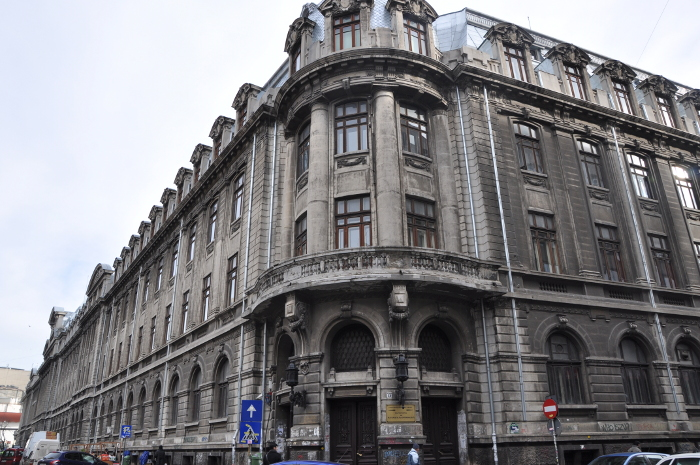
\includegraphics[height=5cm, width=\textwidth]{content_unibuc}
        \label{fig:content_unibuc}
	\end{subfigure}
    \hfill
    \begin{subfigure}[b]{0.3\textwidth}
		\centering
        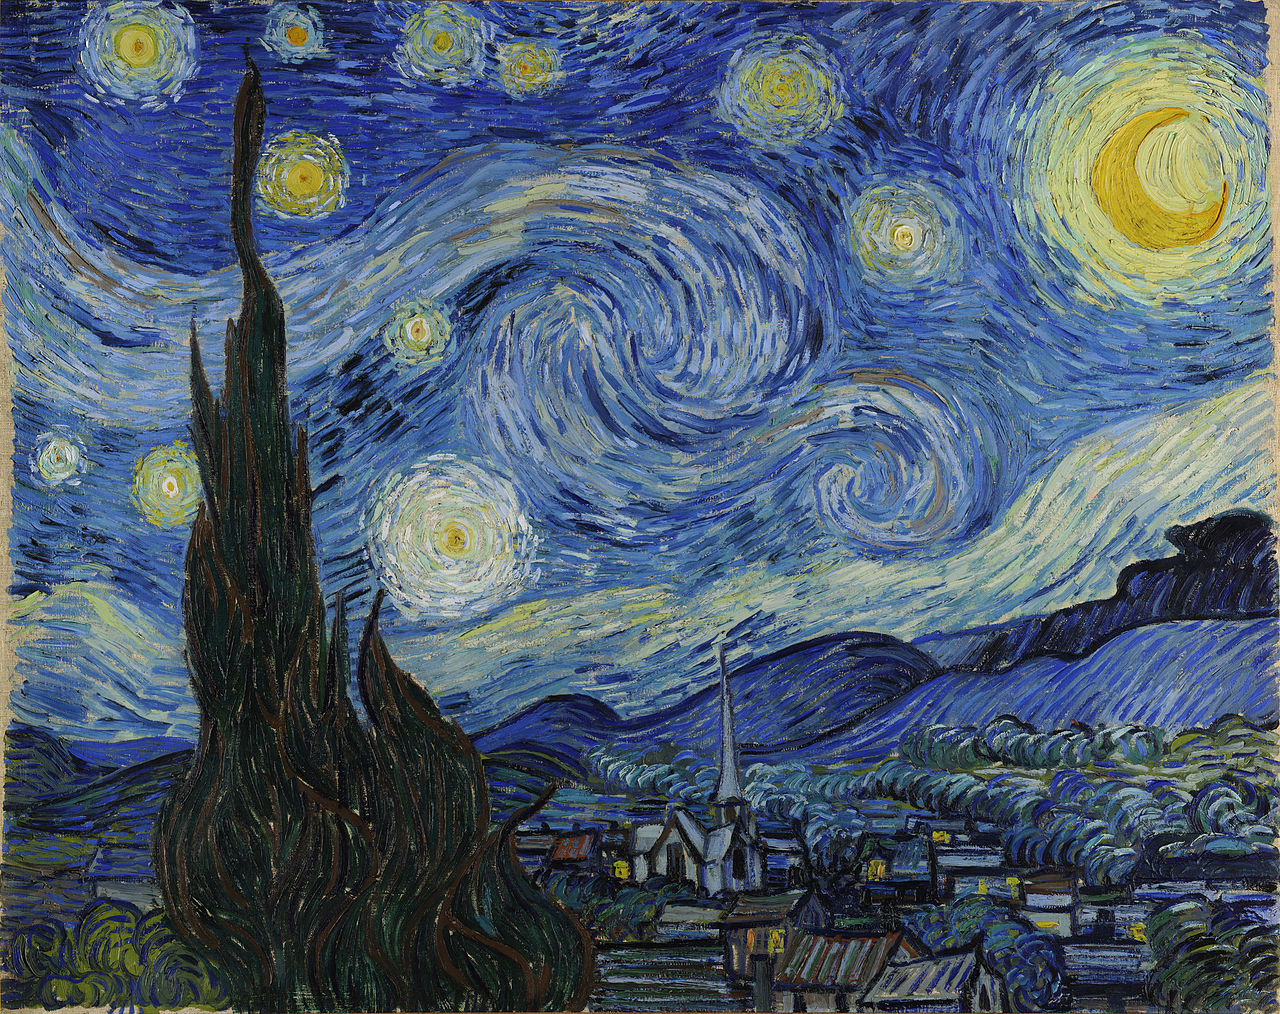
\includegraphics[height=5cm, width=\textwidth]{style1}
        \label{fig:style_unibuc}
	\end{subfigure}
    \hfill
    \begin{subfigure}[b]{0.3\textwidth}
		\centering
        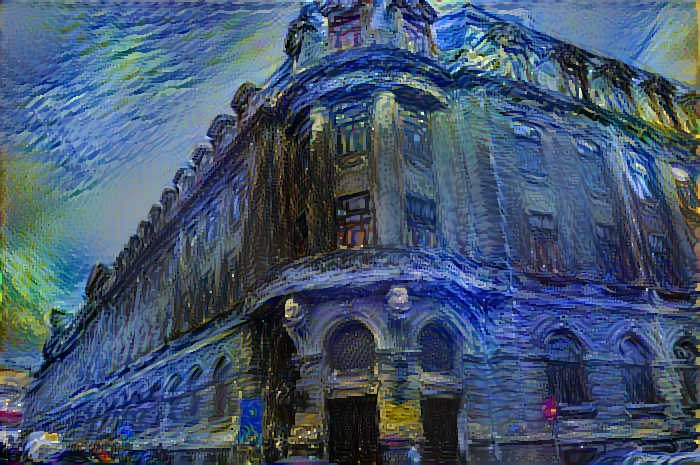
\includegraphics[height=5cm, width=\textwidth]{unibuc}
        \label{fig:content_style_unibuc}
	\end{subfigure}
    \label{fig:unibuc}
\end{figure}

	De-a lungul timpului, oamenii au reușit să altereze mediul înconjurător combinând diferite obiecte cu anumite stiluri, fie ele abstracte sau mai apropiate de realitate, obținând astfel opere de artă. Deși această acțiune este ușor de realizat de către oameni, fiind făcută chiar și de copii, este dificil să se găsească un algoritm care să simuleze acest proces deoarece creierul uman este complex, modul în care funcționează nefiind înțeles în totalitate de către oameni.

\section{Prezentarea lucrării}
În cele ce urmează o să prezint o modalitate pentru rezolvarea problemei din introducere, aceea de a combina conținutul unei poze cu stilul altei poze, obținând astfel poze artistice, asemănătoare cu cele create de om \cite{gatys2015}. Apoi, la această metodă voi adăuga noi constrângeri pentru a putea crea poze cât mai fotografice, de a putea schimba o poză din zi în noapte, de a schimba anotimpul din poză, etc \cite{luan2017}. În final, o să prezint o metodă pentru ca poza dorită să fie creată în timp real deoarece pentru a obține o poză cu metodele anterioare este necesar un timp mai mare de rulare \cite{johnson2016}.

Metodele de mai sus sunt posibile cu ajutorul învățării automate, termen care a fost inventat de către Arthur Samuel în 1959 și care a spus despre învățarea automată: "Un domeniu de studiu care oferă calculatorului abilitatea de a învăța fără a fi explicit programat.", mai exact cu ajutorul rețelelor neurale convoluționale (CNN) [\ref{fig:cnn}]. Având o poză inițializată cu un zgomot aleator sau chiar cu poza în care se află conținutul și o funcție de cost definită pe baza celor trei poze, poza inițială, poza cu conținut și poza cu stil, se vor modifica pixelii din poza inițială astfel încât costul să fie cât mai mic și astfel se va obține o poză artistică având conținutul pozei cu conținut și stilul pozei cu stil.

\begin{figure}[H]
	\centering
	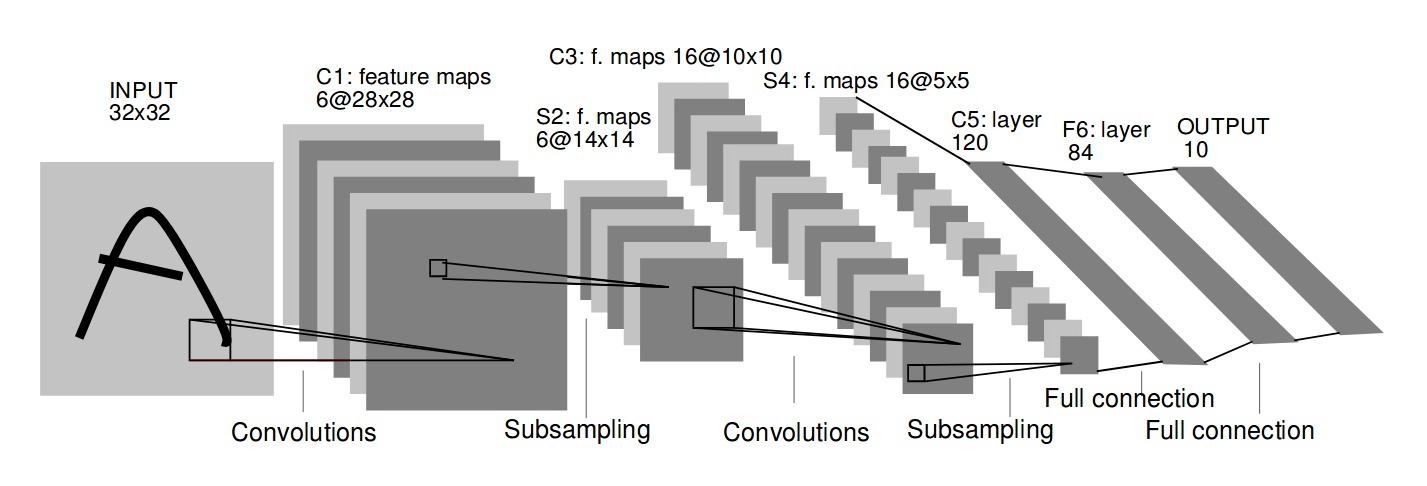
\includegraphics[height=6cm, width=\textwidth]{cnn}
	\caption{Rețea neurală convoluțională \cite{lecun-98}}
	\label{fig:cnn}
\end{figure}

În figura [\ref{fig:cnn}] este prezentă arhitectura unei rețele neurale convoluționale. Acest tip de rețele au adus o îmbunătățire semnificativă în rezolvarea problemelor cu imagini.

Modul în care această rețea merge este unul simplu. La fiecare layer, numit layer convoluțional, sunt definite așa numitele filtre sau kernele de o anumită dimensiune, această dimensiune reprezintă cât de mare este porțiunea din imagine pe care o vede un anumit filtru. Acest filtru, este plimbat pe imagine, de-a lungul tuturor canalelor imaginii, din $n$ în $n$ pixeli și fiecare valoare din filtru este înmulțită cu pixelul corespunzător din porțiunea din imagine, iar apoi aceste valori sunt adunate pentru a obține un singur număr, activarea neuronului. Numerele respective sunt puse într-o matrice ce poartă denumirea de matricea activărilor. Descrierea anterioară se poate vedea mai bine în figura [\ref{fig:filters}].

\begin{figure}[H]
	\centering
	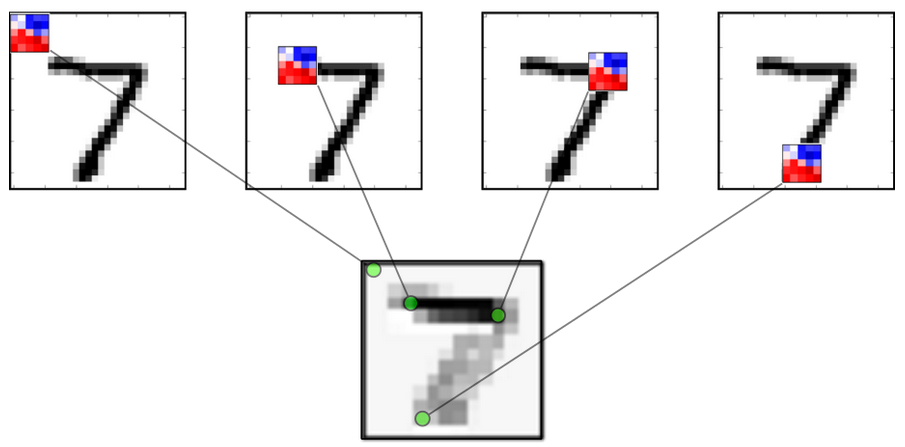
\includegraphics[height=6cm, width=\textwidth]{filters}
	\caption{\cite{filters}}
	\label{fig:filters}
\end{figure}

La un anumit layer există mai multe filtre, fiecare având anumite activări, iar aceste activări sunt așezate ca într-o stivă, precum se poate observa și în figura [\ref{fig:cnn}]. Peste aceste activări este aplicată o funcție neliniară, de obicei ReLU [\ref{sb:relu}] și apoi sunt date ca intrare la următorul layer. Pentru ca rețeaua să învețe caracteristici mai complexe este nevoie ca imaginea inițială să fie micșorată pe parcursul rețelei. Pentru a micșora imaginea sunt posibile mai multe variante, o variantă este de a folosi un tip de layer numit pooling layer. Acesta se bazează pe plimbarea unei ferestre de o anumită dimensiune pe imagine, iar din toți pixelii aflați în fereastră se obține un singur număr reprezentând valoarea maximă a pixelilor sau media tuturor pixelilor [\ref{fig:pool_layer}].

\begin{figure}[h]
	\centering
	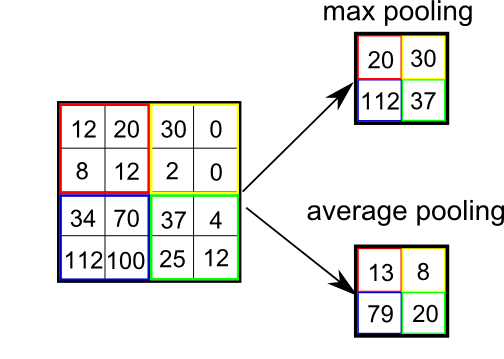
\includegraphics[height=8cm, width=\textwidth]{pool_layer}
	\caption{\cite{pooling}}
	\label{fig:pool_layer}
\end{figure}

O altă variantă de micșorare a pozei este aceea ca atunci când plimbăm filtrul pe o poză, să alegem un număr mai mare de pixeli dintre glisări, astfel încât să obținem o poză mai mică. În figura [\ref{fig:cnn}] mai apar și câteva layere care conțin valorile activărilor puse într-un vector, aceste layere nu păstrează spațialitatea pozei și sunt folosite după aplicarea layerelor convoluționale.

Ponderile filtrelor și al layerelor vectorizate sunt optimizate folosind algoritmul coborârii pe gradient [\ref{sb:gradient_descent}] pe baza unei funcții de cost care se dorește a fi minimizată.

\subsection{Un algoritm neural al stilului artistic}
În acest capitol voi prezenta articolul lui Leon A. Gatys, A Neural Algorithm of Artistic Style \cite{gatys2015}, apărut în anul 2015. Acesta arată pentru prima dată faptul că stilul și conținutul unei poze sunt separabile în cadrul unei rețele neurale convoluționale și astfel, se pot obține poze artistice combinând două poze aleatoare.

\subsection{Transferul stilului artistic fotografic}
În acest capitol voi prezenta articolul lui Fujun Luan, Deep Photo Style Transfer \cite{luan2017}, apărut în anul 2017. Acesta adaugă noi constrângeri metodei lui Leon A. Gatys pentru a obține poze cât mai fotografice, de a schimba o poză din zi în noapte, de a schimba anotimpul din poză, etc.

\subsection{Transferul stilului artistic în timp real}
În acest capitol voi prezenta articolul lui Justin Johnson, Perceptual Losses for Real-Time Style Transfer and Super-Resolution \cite{johnson2016}, apărut în anul 2016. Acesta vine cu o soluție la timpul mare necesar creării unei poze artistice, reducându-l semnificativ antrenând o rețea neurală convoluțională care învață să aplice un anumit stil pe o poză.

\subsection{Compararea metodelor}
În acest capitol voi compara rezultatele obținute de către cele trei metode de mai sus văzând avantajele și dezavantajele pentru fiecare metodă și în ce situații pot fi folosite acestea pentru a obține rezultate satisfăcătoare.

\chapter{Un algoritm neural al stilului artistic}\thispagestyle{fancy}
\label{anaoas}
\section{Introducere}
În anii recenți rețelele convoluționale [\ref{fig:cnn}] s-au dovedit foarte utile în rezolvarea problemelor care conțin imagini. Spre deosebire de rețelele neurale simple, acestea păstrează spațialitatea imaginii și de aceea se comportă mai bine. În anumite sarcini, precum recunoașterea de obiecte dintr-o poza, rețele neurale convoluționale aproape au atins performanța omului în distingerea obiectelor. Pentru o mai bună înțelegere despre cum funcționează aceste rețele voi prezenta un exemplu. \cite{coursera_convnets}\cite{matthew2013} Alegem un neuron dintr-un anumit layer al rețelei și vedem cum arată porțiunea din imagine pentru care activarea acestui neuron este maximă. În imaginile [\ref{fig:cnn_layer1}, \ref{fig:cnn_layer2}, \ref{fig:cnn_layer3}, \ref{fig:cnn_layer4}, \ref{fig:cnn_layer5}], care au fost luate din articolul lui Matthew D. Zeiler, Visualizing and Understanding Convolutional Networks apărut în anul 2013 \cite{matthew2013}, pentru fiecare layer în parte, au fost aleși diferiți neuroni din layer-ul respectiv, iar pentru fiecare neuron, au fost alese noua imagini care maximizează activarea neuronului și afișată porțiunea pe care neuronul respectiv o vede din poza întreagă.
\begin{figure}[h]
	\centering
	\begin{subfigure}[b]{0.4\textwidth}
		\centering
        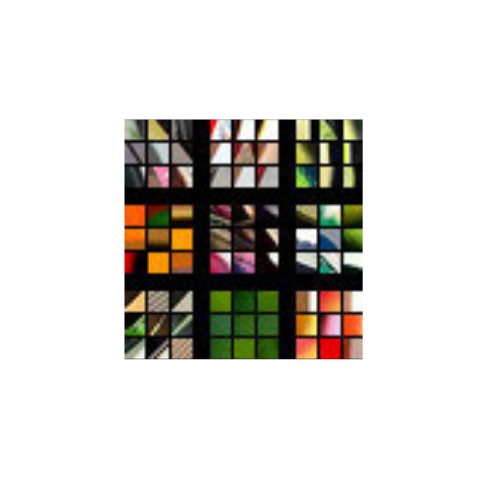
\includegraphics[height=8cm, width=\textwidth]{cnn_layer1}
        \caption{Layer 1. După cum se poate observa în această poză, neuronii din primul layer tind să se activeze la caracteristici precum linii sau anumite nuanțe de culoare. De exemplu, în colțul din stânga sus neuronul respectiv a avut o activare mare la porțiunile din imagine care conțin linii oblice. Pe când, la zona din mijloc de pe ultimul rând, un alt neuron s-a activat când în porțiunea pe care acesta o vede erau diferite nuanțe de verde.}
        \label{fig:cnn_layer1}
	\end{subfigure}
    \hfill
    \begin{subfigure}[b]{0.4\textwidth}
		\centering
        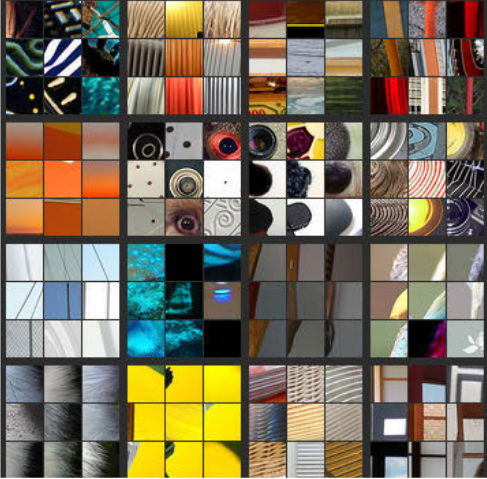
\includegraphics[height=8cm, width=\textwidth]{cnn_layer2}
        \caption{Layer 2. Neuronii din acest layer s-au activat la caracteristici mai complexe decât cele la care s-au activat neuronii din primul layer. Se poate observa de exemplu în poza a doua de pe primul rând că neuronul respectiv s-a activat când a văzut un fel de textură alcătuită din linii. În ultima poză de pe primul rând, neuronul respectiv se uită la acele porțiuni din imagine care conțin o linie verticală în centru.}
        \label{fig:cnn_layer2}
	\end{subfigure}
    \caption{Layer 1 și layer 2}
    \label{fig:cnn_layer1_2}
\end{figure}
\begin{figure}[h]
		\centering
        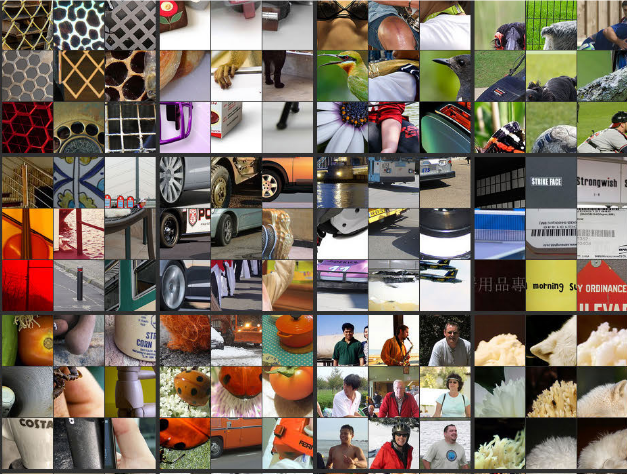
\includegraphics[height=8cm, width=\textwidth]{cnn_layer3}
        \caption{Layer 3. În acest layer de exemplu, în poza din colțul stânga sus, neuronul respectiv detectează un anumit fel de textură. În poza a treia de pe ultimul rând se observă că acel neuron se activează la oameni care stau într-o anumită poziție.}
        \label{fig:cnn_layer3}
\end{figure}
\begin{figure}[h]
	\centering
	\begin{subfigure}[b]{0.4\textwidth}
		\centering
        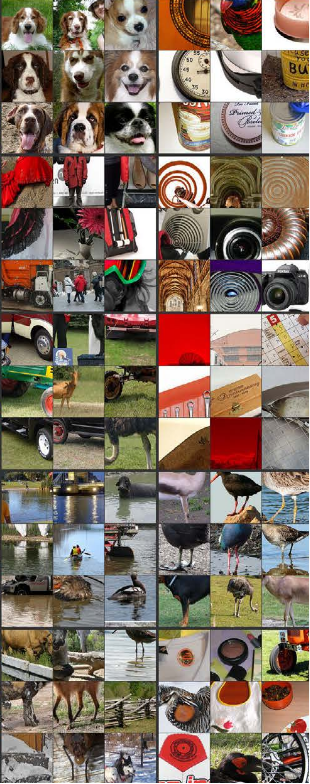
\includegraphics[height=11cm, width=\textwidth]{cnn_layer4}
        \caption{Layer 4. În acest layer de exemplu, în poza din colțul stânga sus se observă că neuronul respectiv a învățat să detecteze o anumită rasă de câini. Pe când neuronul din poza din dreapta de pe al patrulea rând se uită la picioare de animale.}
        \label{fig:cnn_layer4}
	\end{subfigure}
    \hfill
    \begin{subfigure}[b]{0.4\textwidth}
		\centering
        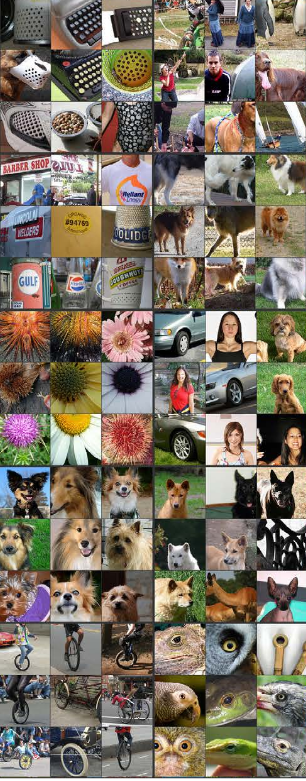
\includegraphics[height=11cm, width=\textwidth]{cnn_layer5}
        \caption{Layer 5. În acest layer de exemplu, în poza din stânga de pe ultimul rând se observă că neuronul respectiv a avut activarea maximă când în poză sunt roți subțiri. Pe când, tot pe acest rând, dar la poza din dreapta, neuronul respectiv se uită la ochi de animale.}
        \label{fig:cnn_layer5}
	\end{subfigure}
    \caption{Layer 4 și layer 5}
    \label{fig:cnn_layer4_5}
\end{figure}

O explicație pentru care caracteristicile la care se activează neuronii din layerele mai adânci sunt mai complexe este aceea că de-a lungul rețelei neurale, poza este micșorată și astfel neuronii văd o porțiune mai mare din imagine. De asemenea, neuronii din fiecare layer se uită la activările neuronilor din layerul precedent, și astfel combinând caracteristici simple se obțin caracteristici mai complexe.

\subsection{Generarea conținutului}
\label{ss:genc}
Din exemplul de mai sus, se observă că atunci când o rețea neurală convoluțională este antrenată să recunoască diferite obiecte dintr-o imagine, aceasta învață să se uite la caracteristici complexe din imagine și astfel este posibil ca având o poză inițializată cu zgomot aleator, o poză oarecare și o funcție de cost bazată pe cele două poze și pe activările neuronilor dintr-un anumit layer, să obținem din poza cu zgomot o poză asemănătoare cu cea pe care o dorim să o recreăm. \cite{mahendran2014} Astfel, bazându-ne pe această ideea putem genera o poză cu conținut asemănător cu cel al unei poze aleatoare alegând un singur layer.

În figura [\ref{fig:content_rec}] se poate observa mai bine ce am spus mai sus. Pe prima coloană se afla poza cu conținut pe care am dorit să o recreez, pe a doua coloană se află imaginea reconstruită, pornind de la o imagine inițializată cu zgomot, iar pe a treia coloană se află o parte din imaginea respectivă pentru a se vedea mai bine detaliile. Pentru poza de la $A$ am folosit activările din layerul \textit{conv1{\_}2}, pentru poza de la $B$ am ales layerul \textit{conv2{\_}2}, pentru poza de la $C$ am ales layerul \textit{conv3{\_}2}, pentru poza de la $D$ am ales layerul \textit{conv4{\_}2}, iar pentru poza de la $E$ am ales layerul \textit{conv5{\_}2}, peste toate aceste activări am aplicat ReLU. Se observă că dacă se generează poza folosind primele layere, atunci pixelii acesteia au aproape aceleași valori ca și pixelii din poza inițială, pe când dacă se generează poza folosind layere aflate mai departe în rețea se păstrează conținutul, dar pixelii sunt diferiți.

\begin{figure}[h]
	\centering
    \begin{subfigure}[b]{0.3\textwidth}
    	A
		\centering
        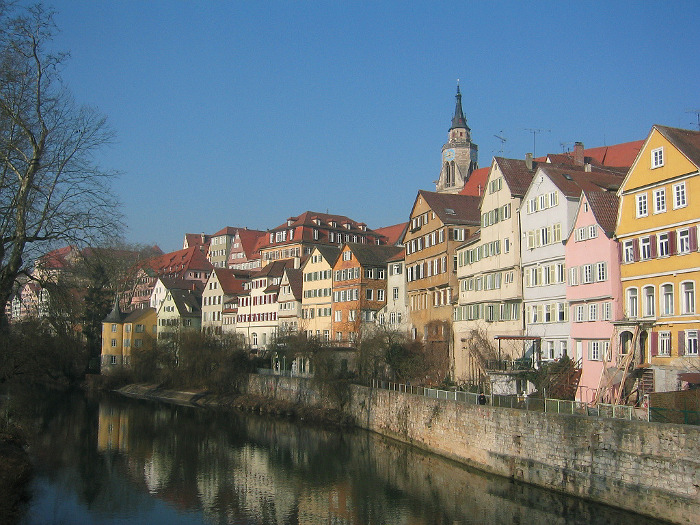
\includegraphics[height=4cm, width=0.9\textwidth]{content1}
        \label{fig:content}
	\end{subfigure}
    \hfill
    \begin{subfigure}[b]{0.3\textwidth}
		\centering
        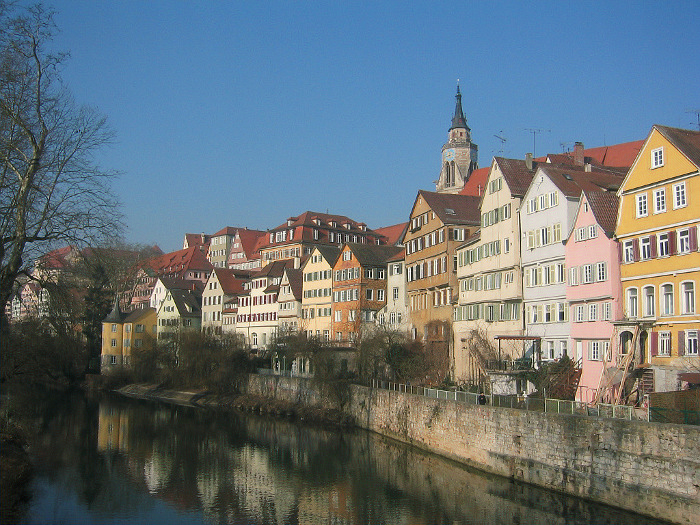
\includegraphics[height=4cm, width=0.9\textwidth]{content_relu1_2}
        \label{fig:content_relu1_2}
	\end{subfigure}
    \hfill
    \begin{subfigure}[b]{0.3\textwidth}
		\centering
        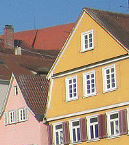
\includegraphics[height=4cm, width=0.9\textwidth]{content_relu1_2_crop}
        \label{fig:content_relu1_2_crop}
	\end{subfigure}
    \begin{subfigure}[b]{0.3\textwidth}
    	B
		\centering
        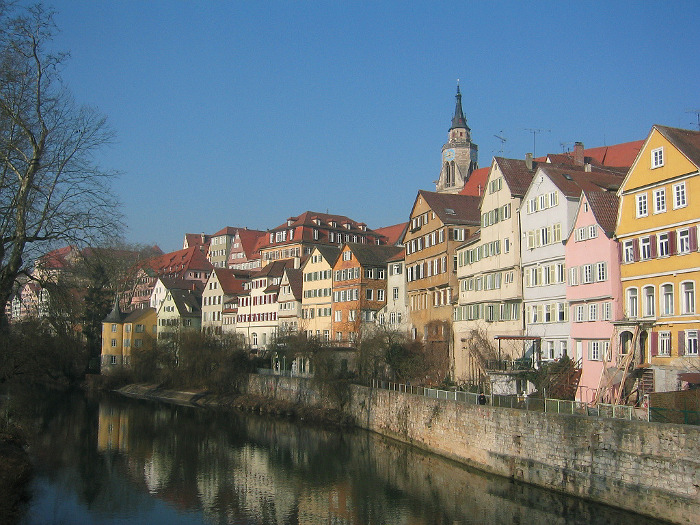
\includegraphics[height=4cm, width=0.9\textwidth]{content1}
        \label{fig:content}
	\end{subfigure}
    \hfill
    \begin{subfigure}[b]{0.3\textwidth}
		\centering
        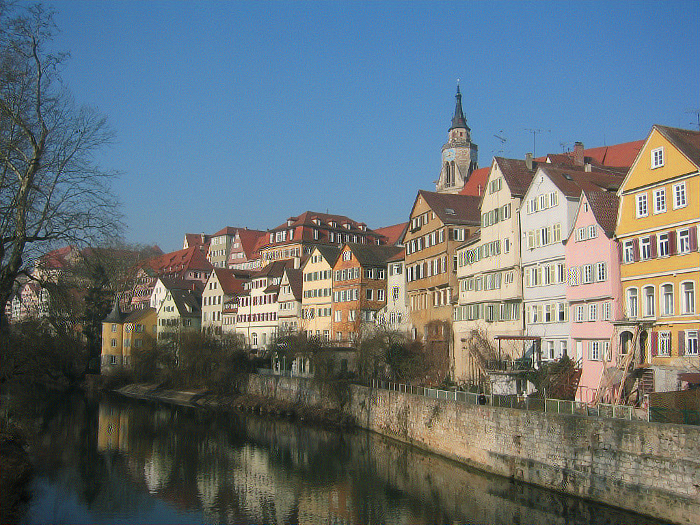
\includegraphics[height=4cm, width=0.9\textwidth]{content_relu2_2}
        \label{fig:content_relu2_2}
	\end{subfigure}
    \hfill
    \begin{subfigure}[b]{0.3\textwidth}
		\centering
        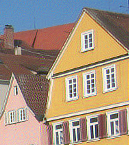
\includegraphics[height=4cm, width=0.9\textwidth]{content_relu2_2_crop}
        \label{fig:content_relu2_2_crop}
	\end{subfigure}
    \begin{subfigure}[b]{0.3\textwidth}
    	C
		\centering
        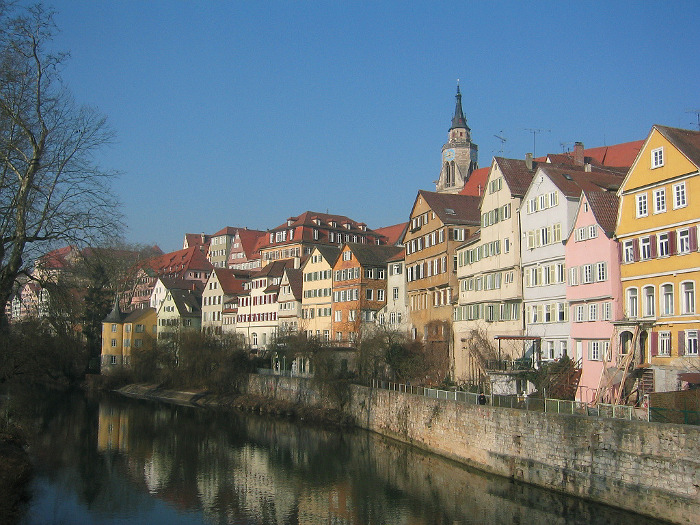
\includegraphics[height=4cm, width=0.9\textwidth]{content1}
        \label{fig:content}
	\end{subfigure}
    \hfill
    \begin{subfigure}[b]{0.3\textwidth}
		\centering
        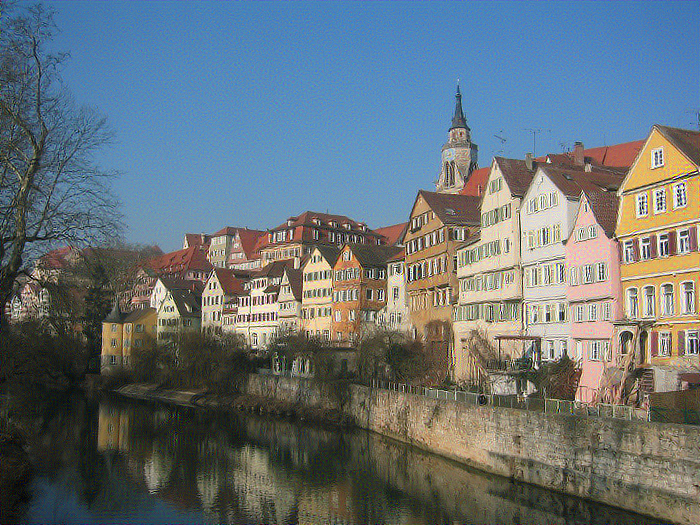
\includegraphics[height=4cm, width=0.9\textwidth]{content_relu3_2}
        \label{fig:content_relu3_2}
	\end{subfigure}
    \hfill
    \begin{subfigure}[b]{0.3\textwidth}
		\centering
        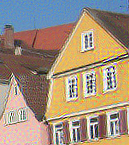
\includegraphics[height=4cm, width=0.9\textwidth]{content_relu3_2_crop}
        \label{fig:content_relu3_2_crop}
	\end{subfigure}
    \begin{subfigure}[b]{0.3\textwidth}
    	D
		\centering
        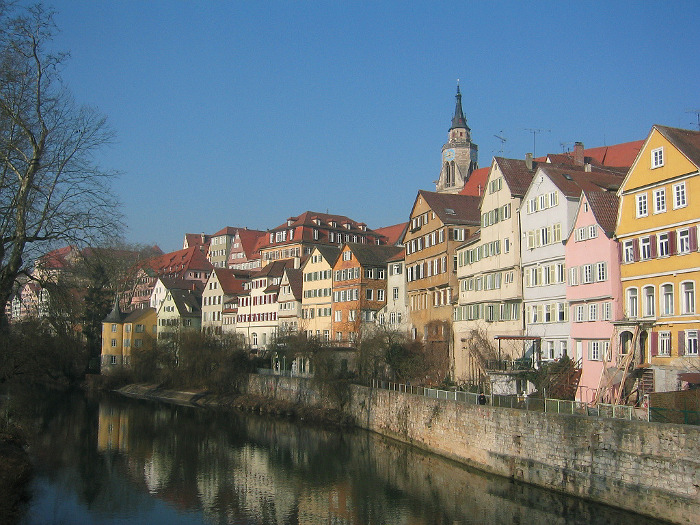
\includegraphics[height=4cm, width=0.9\textwidth]{content1}
        \label{fig:content}
	\end{subfigure}
    \hfill
    \begin{subfigure}[b]{0.3\textwidth}
		\centering
        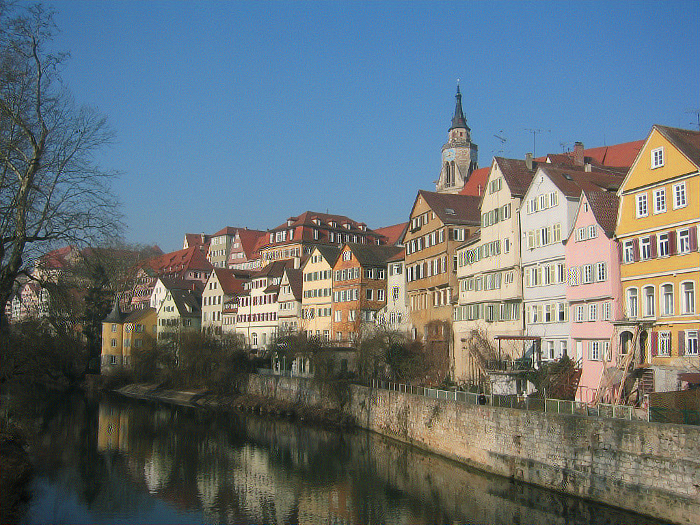
\includegraphics[height=4cm, width=0.9\textwidth]{content_relu2_2}
        \label{fig:content_relu4_2}
	\end{subfigure}
    \hfill
    \begin{subfigure}[b]{0.3\textwidth}
		\centering
        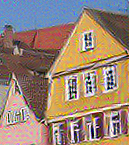
\includegraphics[height=4cm, width=0.9\textwidth]{content_relu4_2_crop}
        \label{fig:content_relu4_2_crop}
	\end{subfigure}
    \begin{subfigure}[b]{0.3\textwidth}
    	E
		\centering
        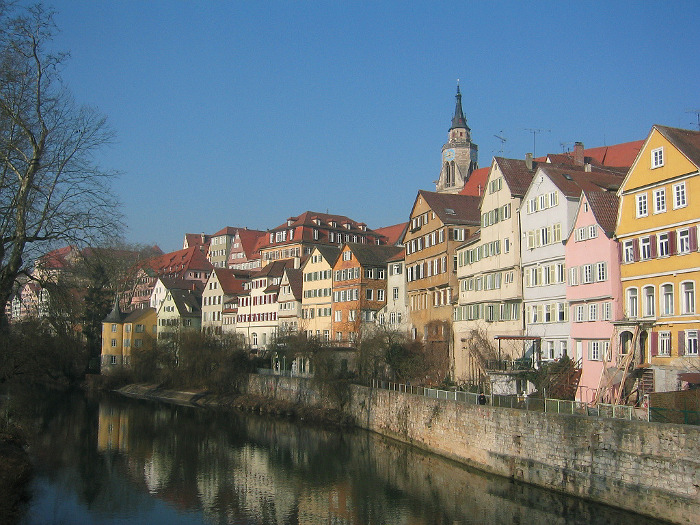
\includegraphics[height=4cm, width=0.9\textwidth]{content1}
        \label{fig:content}
	\end{subfigure}
    \hfill
    \begin{subfigure}[b]{0.3\textwidth}
		\centering
        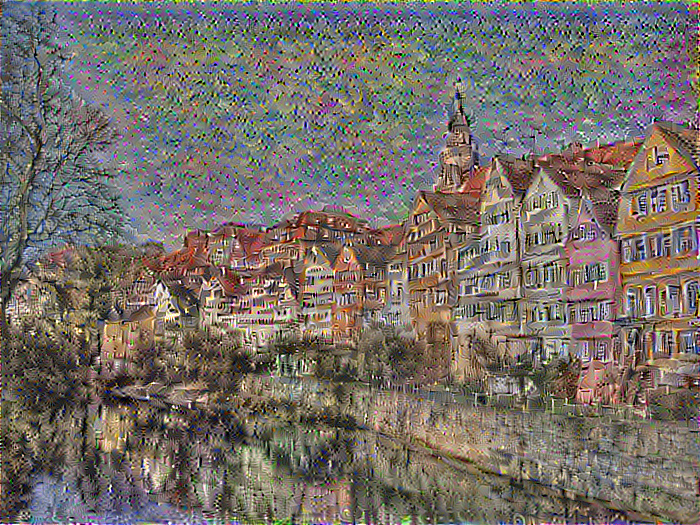
\includegraphics[height=4cm, width=0.9\textwidth]{content_relu5_2}
        \label{fig:content_relu5_2}
	\end{subfigure}
    \hfill
    \begin{subfigure}[b]{0.3\textwidth}
		\centering
        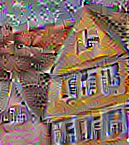
\includegraphics[height=4cm, width=0.9\textwidth]{content_relu5_2_crop}
        \label{fig:content_relu5_2_crop}
	\end{subfigure}
    \caption{Generarea conținutului}
    \label{fig:content_rec}
\end{figure}

\subsection{Generarea stilului}
\label{ss:gens}
După cum am spus, rețelele neurale convoluționale păstrează spațialitatea imaginii și o modelează cu ajutorul filtrelor aplicate asupra acesteia. Dacă atunci când optimizăm o poză cu zgomot, definim o funcție de cost care ține cont de corelația dintre filtrele pozei din unul sau mai multe layere, atunci se obține o textură alcătuită din elemente ale pozei de intrare, precum culoare, linii, diferite forme, etc. \cite{gatys_texture2015}

\begin{figure}[h]
	\centering
    \begin{subfigure}[b]{0.4\textwidth}
    	A
		\centering
        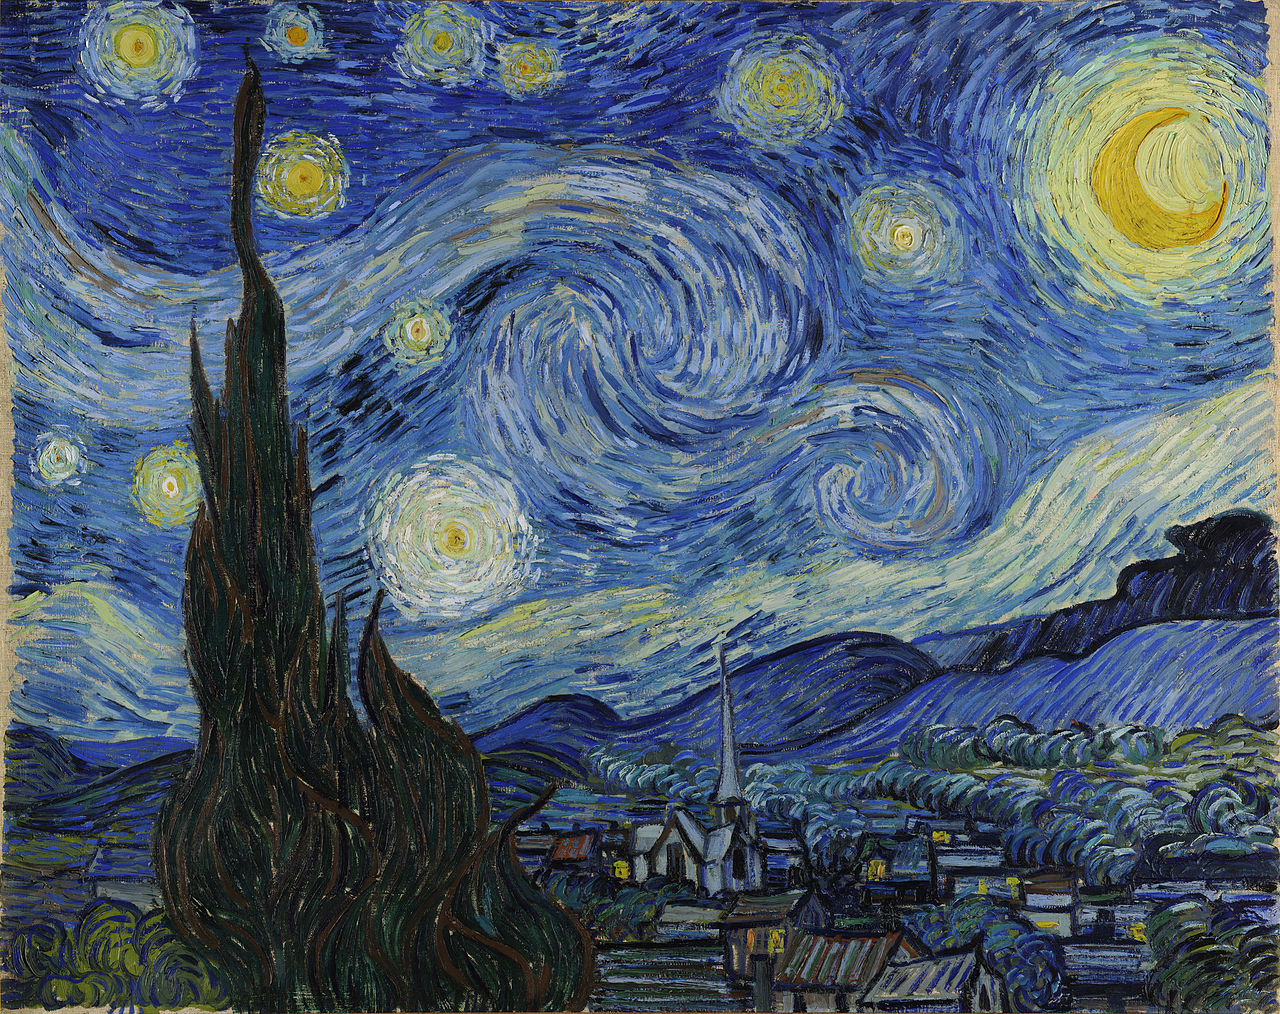
\includegraphics[height=5cm, width=\textwidth]{style1}
        \label{fig:content}
	\end{subfigure}
    \hfill
    \begin{subfigure}[b]{0.4\textwidth}
    	B
		\centering
        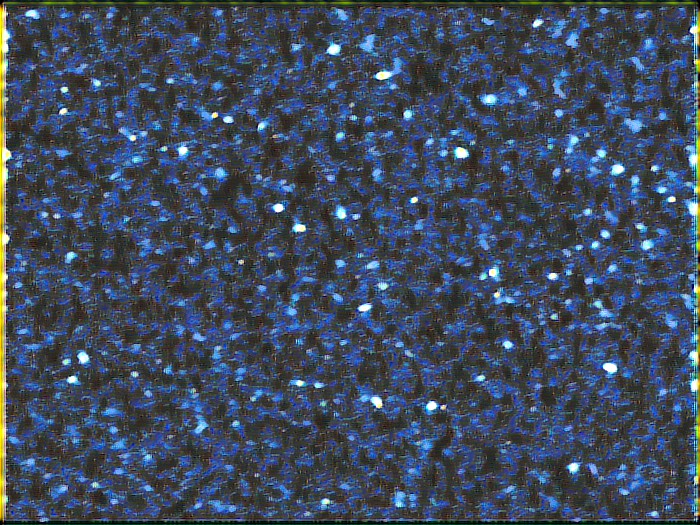
\includegraphics[height=5cm, width=\textwidth]{style_relu1_1}
        \label{fig:style_relu1_1}
	\end{subfigure}
    \begin{subfigure}[b]{0.4\textwidth}
    	C
		\centering
        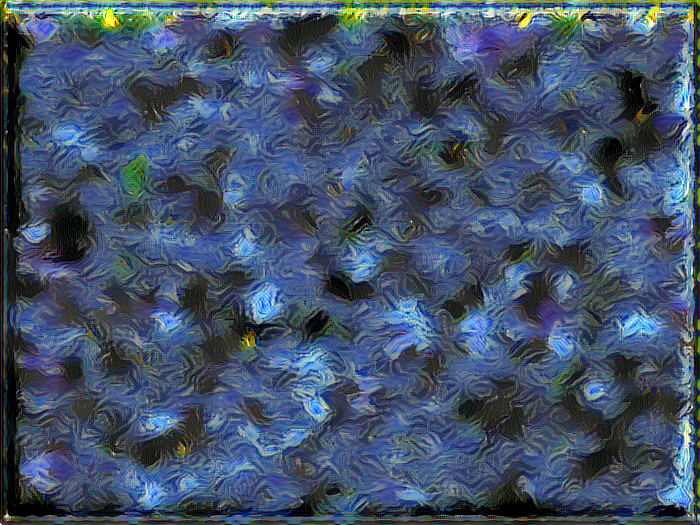
\includegraphics[height=5cm, width=\textwidth]{style_relu2_1}
        \label{fig:style_relu2_1}
	\end{subfigure}
    \hfill
    \begin{subfigure}[b]{0.4\textwidth}
    	D
		\centering
        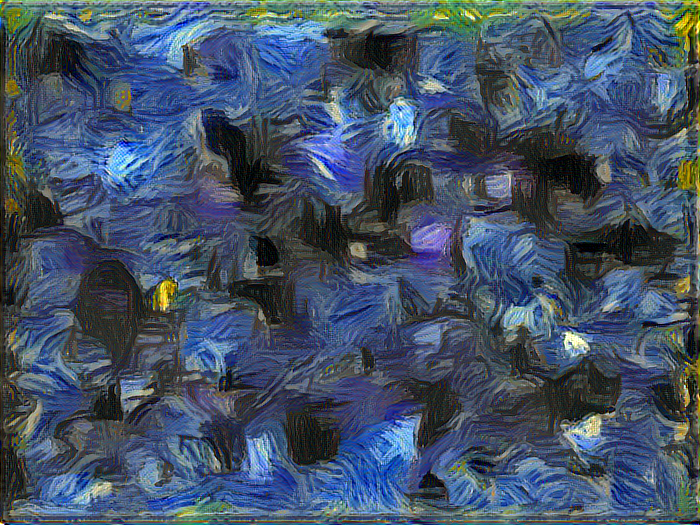
\includegraphics[height=5cm, width=\textwidth]{style_relu3_1}
        \label{fig:style_relu3_1}
	\end{subfigure}
    \begin{subfigure}[b]{0.4\textwidth}
    	E
		\centering
        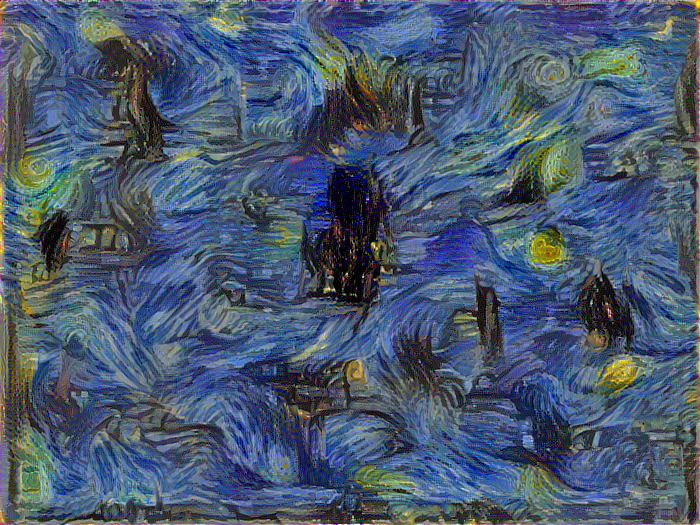
\includegraphics[height=5cm, width=\textwidth]{style_relu4_1}
        \label{fig:style_relu4_1}
	\end{subfigure}
    \hfill
    \begin{subfigure}[b]{0.4\textwidth}
    	F
		\centering
        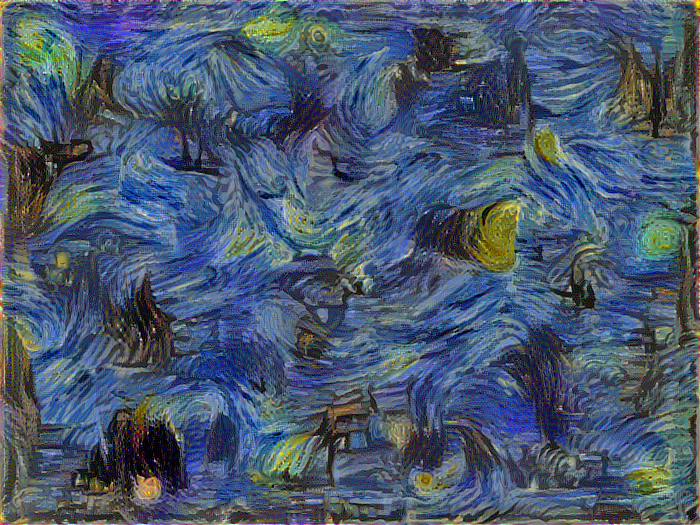
\includegraphics[height=5cm, width=\textwidth]{style_relu5_1}
        \label{fig:content_relu5_1}
	\end{subfigure}
    \caption{Generarea stilului. Figura $A$ este poza pentru care vreau să generez stilul, iar celelalte sunt pozele generate plecând de la o poză inițializată cu zgomot aleator. Pentru poza $B$ am folosit activările din layerul \textit{conv1{\_}1}, pentru poza $C$ am folosit layerele \textit{conv1{\_}1} și \textit{conv2{\_}1}, pentru poza $D$ am folosit layerele \textit{conv1{\_}1}, \textit{conv2{\_}1} și \textit{conv3{\_}1}, pentru poza $E$ am folosit layerele \textit{conv1{\_}1}, \textit{conv2{\_}1}, \textit{conv3{\_}1} și \textit{conv4{\_}1}, iar pentru poza $F$ am folosit layerele \textit{conv1{\_}1}, \textit{conv2{\_}1}, \textit{conv3{\_}1}, \textit{conv4{\_}1} și \textit{conv5{\_}1}. Peste activările acestor layere am aplicat ReLU. Se poate observa că pe măsură ce folosim layere aflate mai departe în rețea, obținem o textură a pozei inițiale, părți din obiectele acesteia apărând în textura generată.}
    \label{fig:style_rec}
\end{figure}

\section{Metodă}
În această secțiune voi defini o funcție de cost, propusă de Leon A. Gatys în articolul sau, A Neural Algorithm of Artistic Style \cite{gatys2015}, care ne va ajuta în generarea unei imagini care combină conținutul unei poze cu stilul alteia.

Această metodă presupune ca având ca date de intrare două poze, o poză în care se află conținutul pe care ni-l dorim în poza finala și o poză care conține stilul dorit să obținem o nouă poză artistică ce combină conținutul cu stilul pozelor de intrare.

Fie $\vec{x}$ o imagine inițializată cu zgomot aleator, $\vec{c}$ imaginea care conține conținutul pe care ni-l dorim și $\vec{s}$ imaginea care conține stilul, atunci $H^l$ este lungimea pozei la layerul $l$, $W^l$ este lățimea pozei la layerul $l$ și $C^l$ este numărul de canale/filtre ale pozei la layerul $l$. $F_{ijk}^l$ este activarea neuronului de la poziția $ijk$ din layerul $l$. Pentru pozele $\vec{x}$ și $\vec{c}$ considerăm matricele activărilor $X_{ijk}^l$, respectiv $C_{ijk}^l$. Atunci, funcția de cost pentru conținut, de care am vorbit în [\ref{ss:genc}] este definită astfel:

\begin{equation}
\label{eq:content_loss}
\mathcal{L}_{continut}(\vec{c}, \vec{x}) = \frac{1}{2H^{l}W^{l}C^{l}} \sum_{i, j, k}{(C_{ijk}^l - X_{ijk}^l)^2}
\end{equation}

La notațiile pentru ecuația [\ref{eq:content_loss}] mai adăugam câteva notații. Fie $N^l$ numărul de filtre pentru o poza din layerul $l$ și $M^l = H^{l} * W^{l}$. Atunci, matricea $FV^l \in \mathcal{R}^{N^{l} \times M^{l}}$ conține pe fiecare linie vectorul filtrului respectiv din layerul $l$, unde $FV_{ij}^l$ este activarea neuronului din filtrul $i$ la poziția $j$ în layerul $l$.

Pentru a putea construi funcția pentru stil, vom folosi matricele gram calculate pentru poza cu zgomot $\vec{x}$, respectiv poza care conține stilul $\vec{s}$. O matrice gram este definită astfel, fie $\vec{v_1}, \vec{v_2} ... \vec{v_n}$ vectori, atunci matricea gram este egală cu produsul scalar dintre fiecare doi vectori $Gram_{ij} = \langle {\vec{v_i}, \vec{v_j}} \rangle$ \cite{wiki_gram}

Pentru pozele $\vec{x}$ și $\vec{s}$ considerăm matricile $XV^l \in \mathcal{R}^{N^{l} \times M^{l}}$, respectiv $SV^l \in \mathcal{R}^{N^{l} \times M^{l}}$ și matricile gram $XG_{ij}^l = \displaystyle \sum_{k}{XV_{ik}^l XV_{jk}^l}$, respectiv $SG_{ij}^l = \displaystyle \sum_{k}{SV_{ik}^l SV_{jk}^l}$.

Pentru o mai bună înțelegere a matricelor gram, se pot vedea pozele [\ref{fig:unrolled_filters}, \ref{fig:gram_matrix}], luate din cursul lui Andrew Ng \cite{coursera_gram}.

\begin{figure}[H]
		\centering
        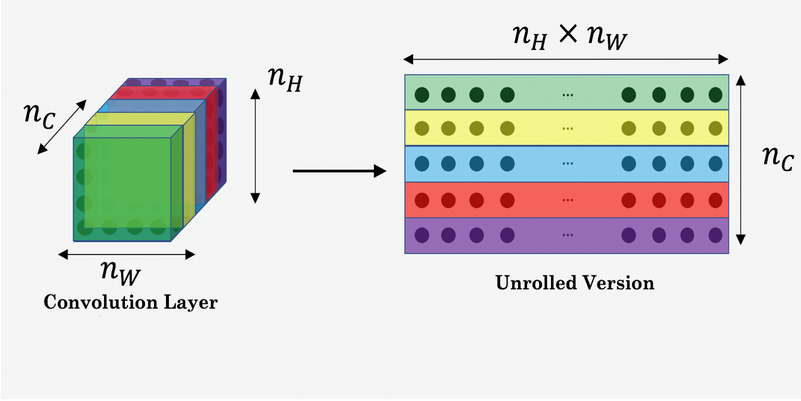
\includegraphics[width=\textwidth]{unrolled_filters}
        \caption{Filtrele salvate ca vectori. $N_H = H^l, N_W = W^l, N_C = C^l$. Aici se poate vedea o exemplificare a matricei $FV^l \in \mathcal{R}^{N^{l} \times M^{l}}$}
        \label{fig:unrolled_filters}
\end{figure}
\begin{figure}[H]
		\centering
        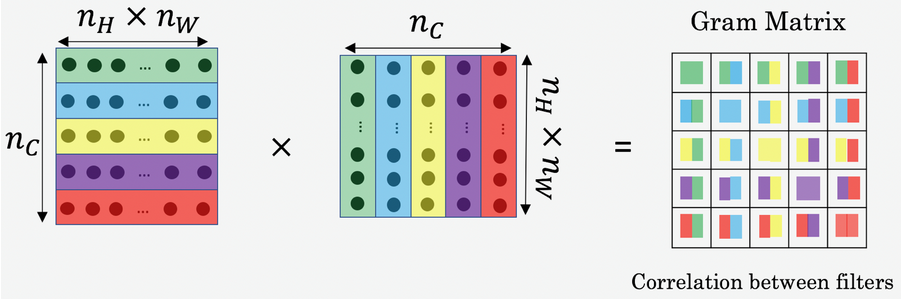
\includegraphics[width=\textwidth]{gram_matrix}
        \caption{Matricea Gram. $N_H = H^l, N_W = W^l, N_C = C^l$. Aici se poate vedea o exemplificare a matricei gram $Gram_{ij} = \langle {\vec{v_i}, \vec{v_j}} \rangle$}
        \label{fig:gram_matrix}
\end{figure}

Așadar, matricea gram calculează cât de mult apar 2 filtre împreuna într-o poza, fiind produsul dintre activările a doi neuroni care văd aceeași porțiune din imagine. Cu cât valoarea din matricea gram este mai mare, cu atât înseamnă că cele două filtre sunt mai corelate.

Având matricele gram calculate, costul dintr-un anumit layer poate fi construit astfel:
\begin{equation}
\label{eq:layer_style_loss}
E_l = \frac{1}{4(H^{l})^{2}(W^{l})^{2}(C^{l})^{2}} \sum_{i, j}{(SG_{ij}^l - XG_{ij}^l)^2}
\end{equation}

Atunci, funcția de cost pentru stil, de care am vorbit în [\ref{ss:gens}] este definită astfel:
\begin{equation}
\label{eq:style_loss}
\mathcal{L}_{stil}(\vec{s}, \vec{x}) = \sum_{l=1}^{L} w_l E_l
\end{equation}
unde $L$ este numărul de layere luate în considerare pentru generarea stilului, iar $w_l$ este un parametru care controlează importanța layerului $l$.

Pentru ca pozele generate să fie cât mai calitative, să nu prezinte zgomot, o să mai definesc o funcție de cost care calculează cât de mult zgomot este în imagine \cite{tvd}. Aceasta are următoarea formulă:

\begin{equation}
\label{eq:tv_loss}
\mathcal{L}_{zgomot}(\vec{x}) = \sum_{i, j} |x_{i+1, j} - x_{i, j}| + |x_{i, j + 1} - x{i, j}|
\end{equation}

Având definite costurile pentru zgomot, conținut și stil, costul total se definește astfel:
\begin{equation}
\label{eq:total_loss}
\mathcal{L}_{total}(\vec{c}, \vec{s}, \vec{x}) = \alpha \mathcal{L}_{continut}(\vec{c}, \vec{x}) + \beta \mathcal{L}_{stil}(\vec{s}, \vec{x}) + \gamma \mathcal{L}_{zgomot}(\vec{x})
\end{equation}
unde parametrii $\alpha$, $\beta$ și $\gamma$ controlează compromisul dintre conținut, stil și respectiv zgomot.

Pe baza funcției totale de cost vom optimiza pixelii unei poze inițializate cu zgomot aleator cu ajutorul algoritmului gradientului de coborâre astfel încât costul total să fie cât mai mic.

\section{Detalii de implementare}
Pentru a implementa metoda descrisă mai sus am folosit Python [\ref{sb:python}] și TensorFlow [\ref{sb:tensorflow}].
După cum am observat, rețelele convoluționale învață anumite reprezentări ale obiectelor dintr-o poză atunci cănd sunt antrenate pentru diferite sarcini. Astfel, pentru a putea calcula costurile definite în subcapitolul precedent ne vom folosi de activările din layerele unei rețele convoluționale care a fost antrenată să recunoască obiectele dintr-o poză. Antrenarea a avut loc pe baza a aproximativ 1,2 milioane de poze, obiectele din poze fiind clasificate în 1000 de categorii. În figura [\ref{fig:imagenet}] se pot observa câteva poze din setul de antrenare. Această rețea a fost folosită la competiția ImageNet din 2014 [\ref{sb:imagenet}], unde a obținut locul 2 la problema de clasificare, obținând o eroare egală cu $0.07$ și se numește VGG19 [\ref{fig:vgg19}], iar parametrii pe care i-a învățat rețeaua în timpul antrenării sunt făcuți publici de către autorii acesteia pe site-ul lor. \cite{parametri_vgg19} Din această rețea am folosit doar layerele convoluționale, fără cele conectate complet, iar în loc de \textit{maxpool} am folosit \textit{avgpool}, precum Leon A. Gatys, deoarece acesta a observat că această modificare produce rezultate mai satisfăcătoare.

\begin{figure}[H]
		\centering
        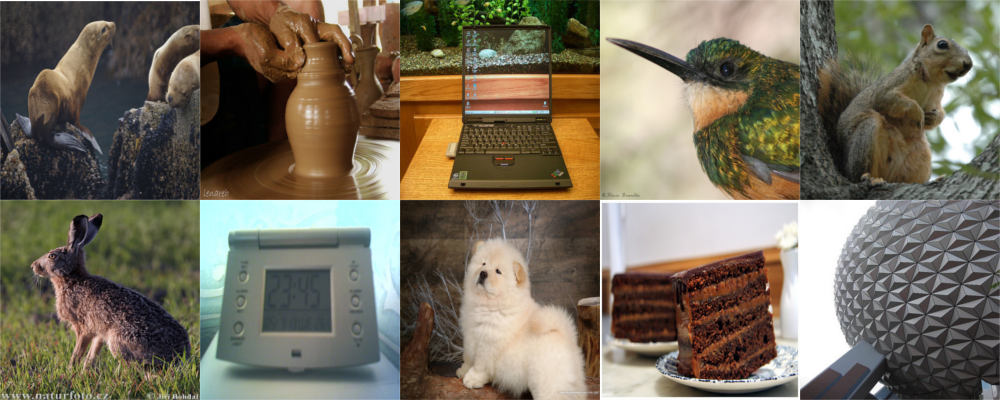
\includegraphics[height=5cm,width=\textwidth]{imagenet}
        \caption{Imagini din setul de antrenare ImageNet}
        \label{fig:imagenet}
\end{figure}

\begin{figure}[H]
		\centering
        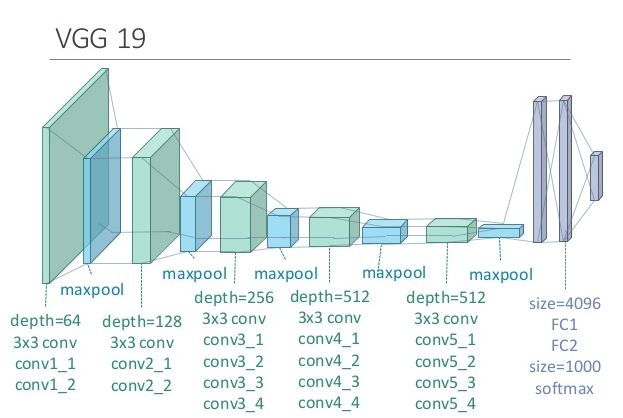
\includegraphics[height=6cm,width=\textwidth]{vgg19}
        \caption{Arhitectura rețelei neurale convoluționale VGG19 \cite{arh_vgg19}}
        \label{fig:vgg19}
\end{figure}

Algoritmul primește ca date de intrare două poze în spațiul de culori RGB, una cu conținutul dorit și alta cu stilul dorit. Având rețeaua de mai sus și cele două poze, am inițializat o poză de aceeași dimensiune cu cea a pozei de conținut folosind inițializarea Xavier [\ref{sb:xavier}], astfel, poza inițială prezintă zgomot aleator, pixelii acesteia având o distribuție uniformă, cu valori între $[-limita, limita]$, unde $limita = \sqrt{\frac{6}{H * W * C}}$, iar $H$ este lungimea pozei, $W$ este lățimea pozei și $C$ este numărul de canale ale pozei.

Apoi am normalizat cele trei poze pentru a avea aceeași distribuție ca cea pe care a fost antrenată rețeaua, și anume, pentru fiecare canal al pozei am scăzut valorile $[123.68, 116.779, 103.939]$, valori care reprezintă media canalelor RGB pentru pozele folosite la antrenare de rețeaua VGG19 și le-am trecut pe rând prin rețea și pentru fiecare am salvat ieșirile din layerul \textit{conv4{\_}2} pentru conținut și ieșirile din layerele \textit{conv1{\_}1}, \textit{conv2{\_}1}, \textit{conv3{\_}1}, \textit{conv4{\_}1}, \textit{conv5{\_}1} pentru stil. Acestea sunt numele layerelor din rețeaua VGG19. Peste aceste valori pe care le-am salvat am aplicat ReLU [\ref{sb:relu}] și am calculat costul cu ajutorul funcțiilor de cost definite, iar cu algoritmul gradientului de coborâre [\ref{sb:gradient_descent}] și a metodei backpropagation [sb:backpropagation] de calculare a gradienților am optimizat pixelii pozei inițiale astfel încât costul total să fie cât mai mic.

În imaginea [\ref{fig:vgg_workflow}] se poate observa procesul pe care l-am descris mai sus.

\begin{figure}[H]
		\centering
        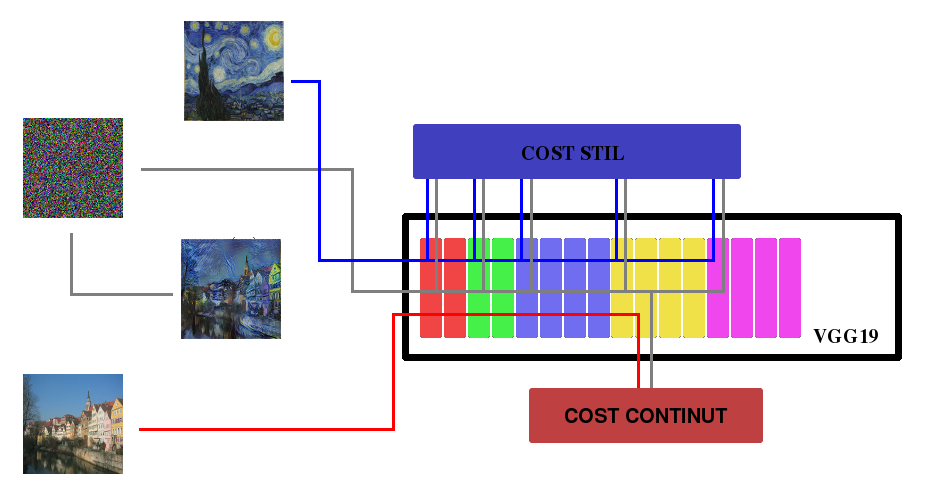
\includegraphics[width=\textwidth]{vgg_workflow}
        \caption{Workflow-ul algoritmului}
        \label{fig:vgg_workflow}
\end{figure}

Pentru toate rezultatele din acest capitol am repetat procedeul de mai sus timp de 2000 de iterații cu rata de învățare [\ref{sb:learning_rate}] egală cu 2 pentru a ajunge la rezultate satisfăcătoare. De asemenea, am ales $\alpha = 100$, $\beta = 1$, $\gamma = 0.03$ și $w_l = 0.2$ pentru toate layerele. Acești parametri i-am ales după mai multe încercări, în care am analizat pozele generate, după percepția mea, deoarece pentru acest timp de problemă nu există o metrică pentru a spune cât de bune sunt pozele generate. Pozele au fost redimensionate, păstrând raportul dintre lungime și lățime, la $max(lungime, latime) = 700$ de pixeli.

\subsection{Python}
\label{sb:python}
Python \cite{wiki_python} este un limbaj de programare, creat de Guido van Rossum în anul 1991. Este suportat de mai multe sisteme de operare fiind un limbaj de programare ușor  de folosit și care oferă posibilitatea de a scrie programe complexe, într-o maniera elegantă. Python este folosit de majoritatea celor care doresc să creeze programe ce folosesc învățarea automată.

\subsection{TensorFlow}
\label{sb:tensorflow}
TensorFlow \cite{wiki_tf} a fost creat de către cercetătorii din echipa Google Brain. Această librărie, prin funcțiile pe care le deține, ca de exemplu calcularea gradienților sau crearea de layere într-o rețea, oferă posibilitatea de a construi ușor programe ce folosesc învățarea automată. Tensorflow este folosit activ de cei de la Google și de asemenea este și open-source, fapt ce constituie un plus, deoarece datorită numărului mare de contribuitori este îmbunătățit continuu.

\subsection{ImageNet}
\label{sb:imagenet}
ImageNet \cite{imagenet} este o bază de date ce conține milioane de poze adnotate de către oameni, imagini destinate pentru diferite probleme legate de învățarea automată. Începând cu anul 2010, în fiecare an se organizează un concurs numit ImageNet Large Scale Visual Recognition Challenge (ILSVRC) în care diferiți cercetători încearcă să obțină rezultate cât mai bune la probleme de genul: clasificarea obiectelor dintr-o poză sau localizarea obiectelor.

\subsection{Inițializarea Xavier}
\label{sb:xavier}
\cite{coursera_deep_learning} O problemă cu care se confruntă rețelele convoluționale foarte adânci este modul în care sunt inițializate filtrele. Dacă acestea sunt inițializate cu valori prea mici, atunci de-a lungul rețelei, este posibil să devină foarte aproape de zero, astfel rețeaua nemaiputând învăța. Pe de altă parte, dacă sunt prea mari, atunci acestea tind să devină prea mari de-a lungul rețelei ca să mai fie folositoare. În articolul său \cite{glorot2010}, Xavier Glorot propune o formulă de inițializare a filtrelor care s-a dovedit a fi fiabilă în practică. Această inițializare are rolul de a ține valorile dintr-un anumit filtru într-un anumit interval, valorile având o distribuție uniformă sau normală. Formula pentru variație în cazul când dorim ca valorile să aibă o distribuție uniformă este:

\begin{equation}
\label{eq:xavier}
variatie = \sqrt{\frac{6}{intrari + iesiri}}
\end{equation}

Unde $intrari$ reprezintă câte valori intră în layerul respectiv, iar $iesiri$ câte valori ies din layerul respectiv.

\subsection{ReLU}
\label{sb:relu}
Rectified linear unit (ReLU) \cite{wiki_relu} este o funcție de activare neliniară. Aceasta se aplică pe valorile de ieșire ale layerelor. Este inspirată din biologie și din cum se crede că funcționează transmiterea de informație în creier. Atunci când un neuron are o valoare negativă, după aplicarea funcției ReLU acesta are valoarea 0, însemnând ca este inactiv, iar când valoarea unui neuron este pozitivă, activarea acestuia este fix valoarea lui.

\begin{equation}
\label{eq:relu}
f(x) = max(0, x)
\end{equation}

\subsection{Coborâre pe gradient}
\label{sb:gradient_descent}
Coborârea pe gradient \cite{coursera_deep_learning} este un algoritm de minimizare a unei funcții care depinde de mai multe variabile. Să presupunem că funcția de cost este următoarea $\mathcal{L}(x_1, x_2 ... x_n)$. Atunci, pentru a minimiza această funcție vom aplica următorul algoritm pentru modificarea variabilelor de care depinde.

\begin{equation}
\label{eq:gradient_descent}
x_i = x_i - \alpha * \frac{\partial}{\partial{x_i}}\mathcal{L}
\end{equation}

Unde $\frac{\partial}{\partial{x_i}}\mathcal{L}$ este derivata parțială a funcției $\mathcal{L}$ în raport cu variabila $x_i$. Derivata reprezintă panta tangentei la graficul funcției, și indică direcția funcției, dacă aceasta crește sau descrește. Iar $\alpha$ este rata de învățare.

\subsection{Backpropagation}
\label{sb:backpropagation}
\cite{coursera_deep_learning} Așa cum am văzut la algoritmul coborârii pe gradient, pentru a minimiza o funcție de cost $\mathcal{L}(x_1, x_2 ... x_n)$, este nevoie să calculăm derivatele parțiale $\frac{\partial}{\partial{x_i}}\mathcal{L}$. Plecând de la rezultatul funcției de cost, cu ajutorul acestei metode se propagă înapoi în rețea eroarea până la variabilele de care depinde această funcție care sunt optimizate după formula [\ref{eq:gradient_descent}].

\subsection{Optimizatorul Adam}
\label{sb:adam_optimizer}
Optimizatorul Adam \cite{coursera_deep_learning} este o variantă îmbunătățită a algoritmului coborârii pe gradient făcând ca învățarea să meargă mai repede. O problemă a coborârii pe gradient este aceea că face mulți pași până a ajunge să conveargă către minim. Optimizatorul Adam se folosește de valorile anterioare ale gradienților, și intuitiv, vede un trend pe care îl urmează gradienții, putând la un anumit moment să facă un pas mai mare decât ar face algoritmul coborârii pe gradient. Formula acestuia la pasul $t$ este următoarea:

\begin{equation}
V_t = \beta1 * V_{t-1} + (1 - \beta1) * \frac{\partial}{\partial{x_i}}\mathcal{L}
\end{equation}
\begin{equation}
S_t = \beta2 * S_{t-1} + (1 - \beta2) * \frac{\partial}{\partial{x_i}}\mathcal{L} * \frac{\partial}{\partial{x_i}}\mathcal{L}
\end{equation}
\begin{equation}
\label{eq:adam}
x_i = x_i - \alpha * \frac{V_t}{\sqrt{S_t} + \epsilon}
\end{equation}

Unde, de obicei, $\beta1 = 0.9$, asta însemnând aproximativ că $V_t$ calculează media ultimilor 10 gradienți, $\beta2 = 0.999$, $\epsilon = 1e-08$, acesta este folosit în cazul în care $S_t = 0$ și să se evite împărțirea la 0, iar $\alpha$ este rata de învățare.

\subsection{Rata de învățare}
\label{sb:learning_rate}
Rata de învățare \cite{coursera_deep_learning} este folosită în formula algoritmilor de optimizare. Aceasta controlează cat de mult să fie modificată o variabilă pentru a optimiza funcția țintă. O valoare mica a acestei rate, înseamnă că variabila respectivă se va modifica foarte puțin, fiind necesar un timp mai mare pentru ca funcția să conveargă către minim. Pe de altă parte, dacă rata de învățarea este foarte mare, atunci este posibil ca funcția să nu mai ajungă să conveargă, deoarece variabila este modificată foarte mult.

\newpage
\section{Rezultate și comparații}
\begin{figure}[H]
	\centering
    \begin{subfigure}[b]{0.75\textwidth}
		\centering
        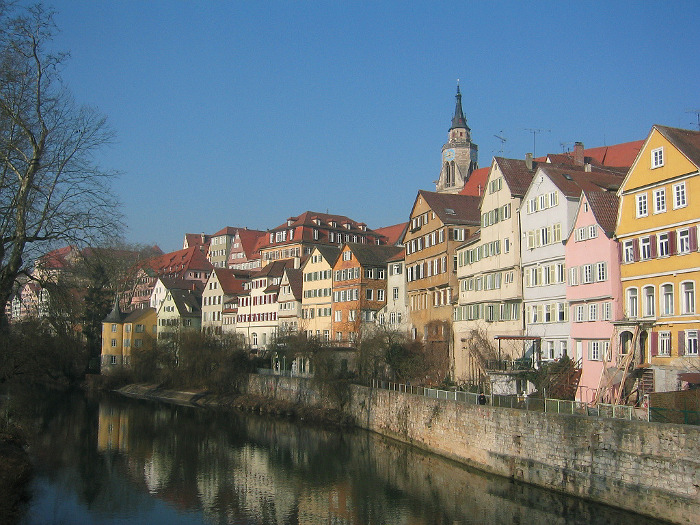
\includegraphics[height=4.5cm, width=0.7\textwidth]{content1}
        \label{fig:content}
        \caption{Neckarfront, Tübingen, Germania, autor Andreas Praefcke.}
	\end{subfigure}
    \begin{subfigure}[b]{0.5\textwidth}
		\centering
        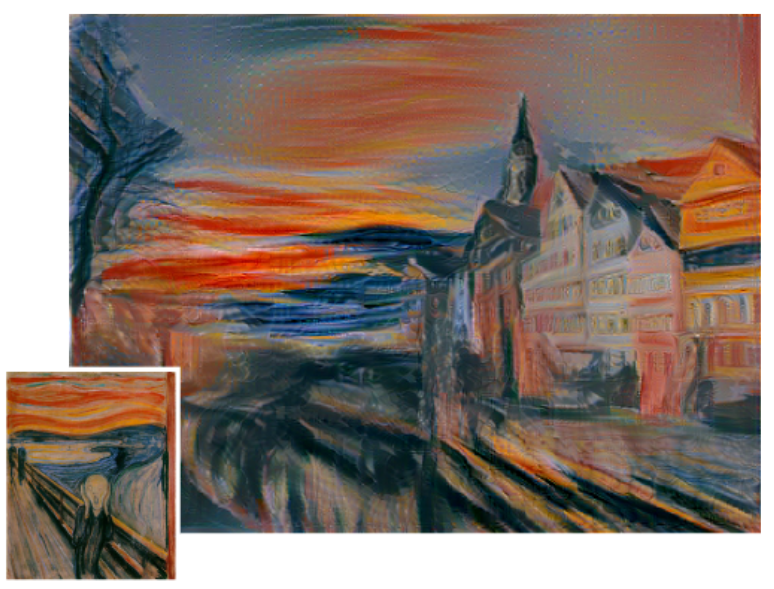
\includegraphics[height=4.5cm, width=1.1\textwidth]{anaoas_c1s2_gatys}
        \label{fig:anaoas_c1s2_gatys}
        \caption{The Scream, Edvard Munch, 1893.}
	\end{subfigure}
    \hfill
    \begin{subfigure}[b]{0.4\textwidth}
		\centering
        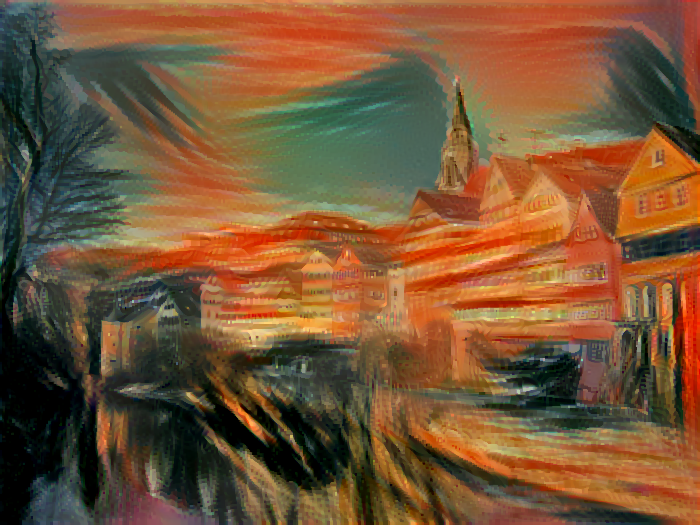
\includegraphics[height=4.5cm, width=1.2\textwidth]{anaoas_c1s2}
        \label{fig:anaoas_c1s2}
	\end{subfigure}
    \begin{subfigure}[b]{0.5\textwidth}
		\centering
        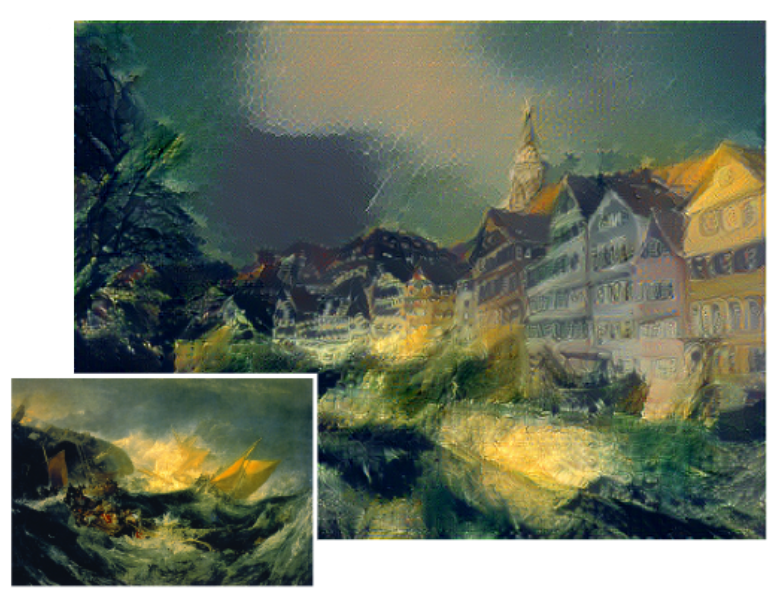
\includegraphics[height=4.5cm, width=1.1\textwidth]{anaoas_c1s3_gatys}
        \label{fig:anaoas_c1s3_gatys}
        \caption{The Shipwreck of the Minotaur, J.M.W. Turner, 1805}
	\end{subfigure}
    \hfill
    \begin{subfigure}[b]{0.4\textwidth}
		\centering
        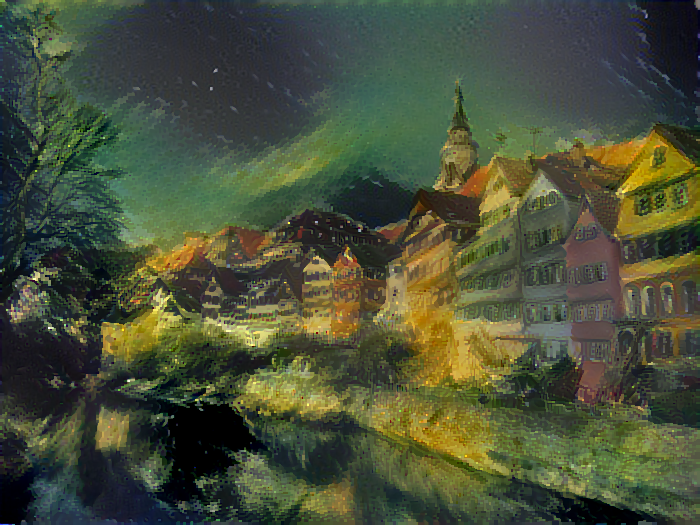
\includegraphics[height=5cm, width=1.2\textwidth]{anaoas_c1s3}
        \label{fig:anaoas_c1s3}
	\end{subfigure}
    \caption{Pe coloana din stânga sunt rezultatele luate din articolul lui Leon A. Gatys, iar pe coloana din dreapta sunt rezultatele obținute de mine. Pozele diferă deoarece contează dimensiunea imaginilor între care s-a realizat transferul de stil sau modul în care a fost implementat algoritmul. Fiindcă nu există un mod obiectiv pentru a decide care imagini sunt mai artistice, ambele variante sunt valabile.}
\end{figure}

\begin{figure}[H]
	\centering
    \begin{subfigure}[b]{0.5\textwidth}
		\centering
        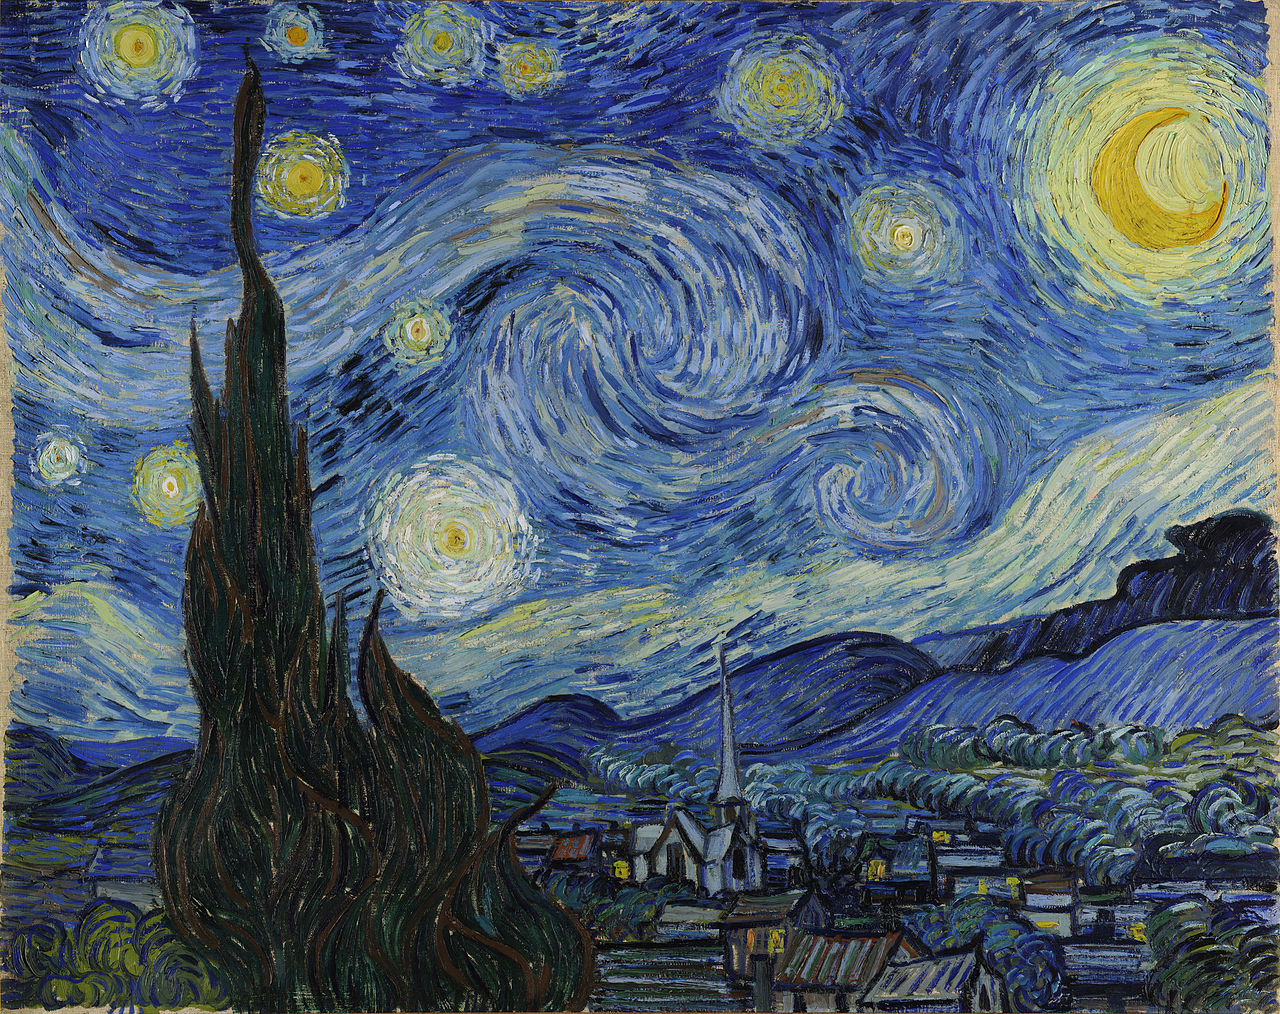
\includegraphics[height=2.5cm, width=0.7\textwidth]{style1}
        \label{fig:anaoas_style1}
        \caption{The Starry Night, Vincent van Gogh, 1889}
	\end{subfigure}
    \hfill
    \begin{subfigure}[b]{0.4\textwidth}
		\centering
        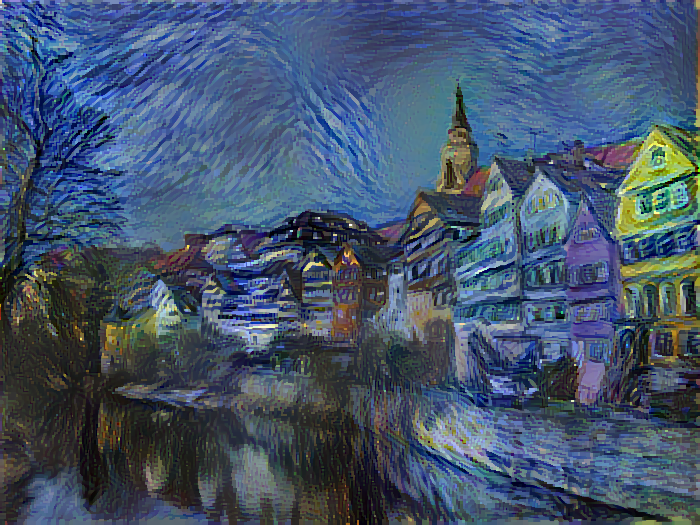
\includegraphics[height=4cm, width=1.1\textwidth]{anaoas_c1s1}
        \label{fig:anaoas_c1s1}
	\end{subfigure}
    \begin{subfigure}[b]{0.5\textwidth}
		\centering
        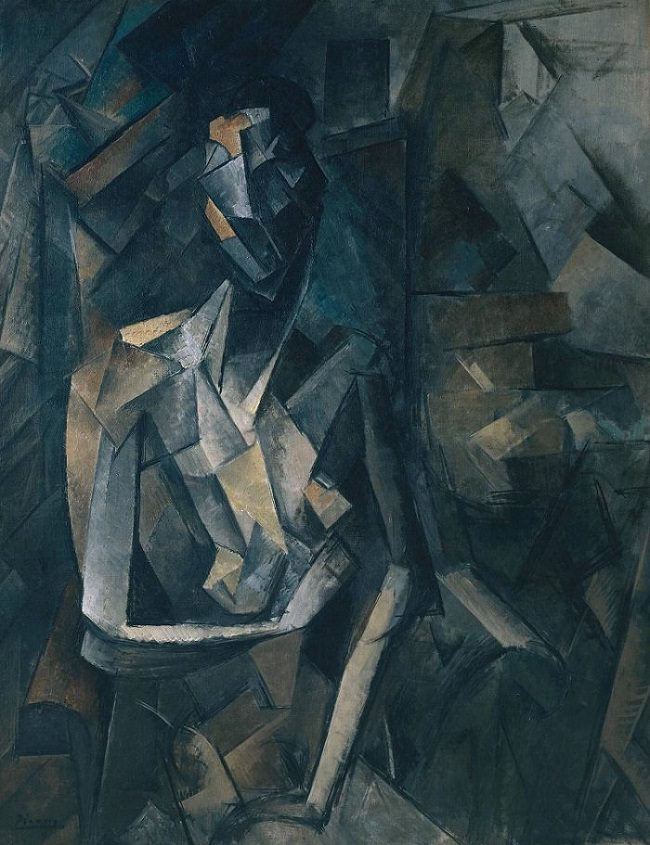
\includegraphics[height=2.5cm, width=0.7\textwidth]{style4}
        \label{fig:anaoas_style4}
        \caption{Femme nue assise, Pablo Picasso, 1910}
	\end{subfigure}
    \hfill
    \begin{subfigure}[b]{0.4\textwidth}
		\centering
        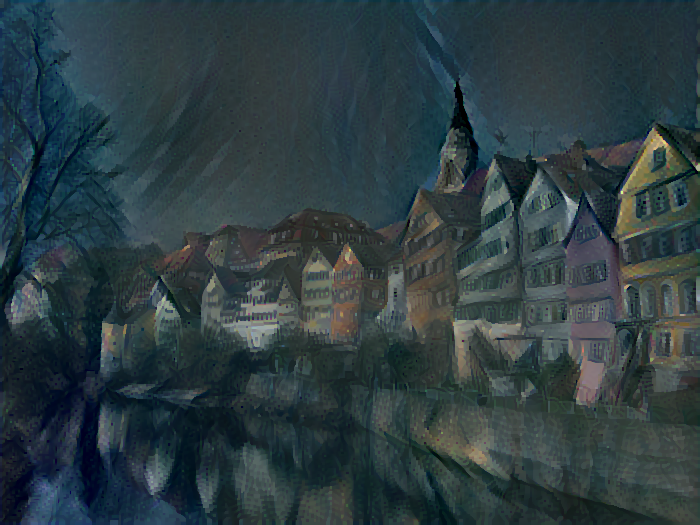
\includegraphics[height=4cm, width=1.1\textwidth]{anaoas_c1s4}
        \label{fig:anaoas_c1s4}
	\end{subfigure}
    \begin{subfigure}[b]{0.5\textwidth}
		\centering
        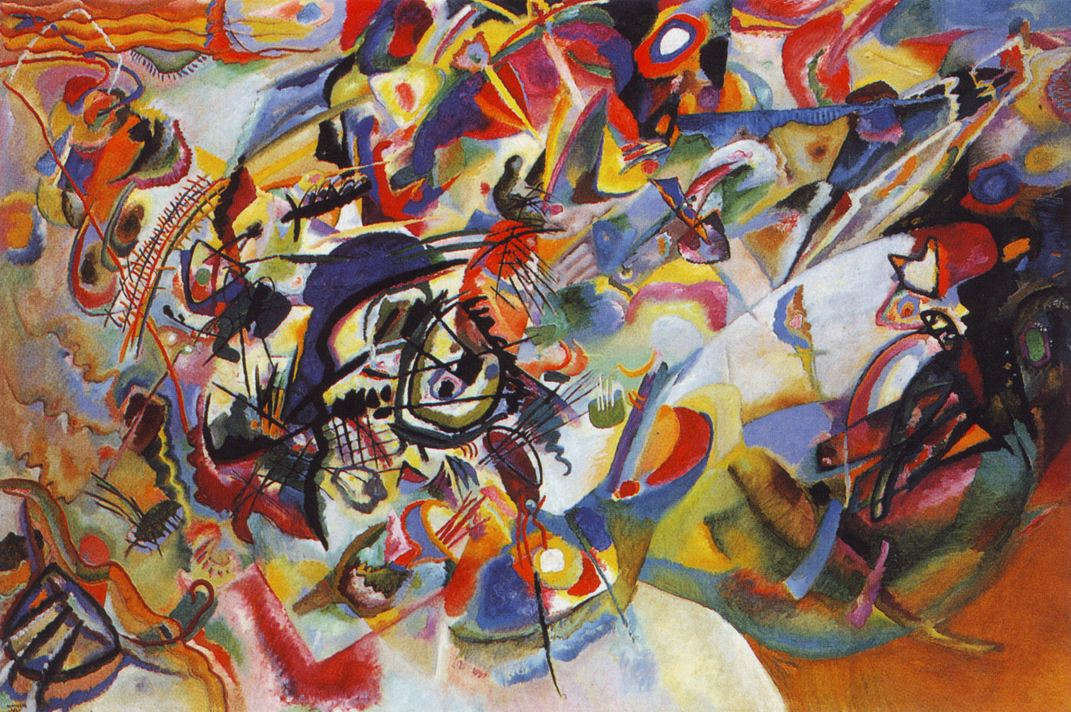
\includegraphics[height=2.5cm, width=0.7\textwidth]{style5}
        \label{fig:anaoas_style5}
        \caption{Composition VII, Wassily Kandinsky, 1913}
	\end{subfigure}
    \hfill
    \begin{subfigure}[b]{0.4\textwidth}
		\centering
        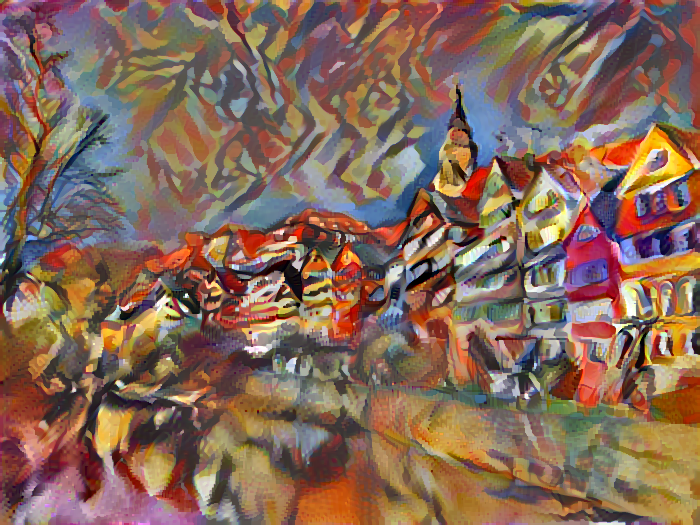
\includegraphics[height=4cm, width=1.1\textwidth]{anaoas_c1s5}
        \label{fig:anaoas_c1s5}
	\end{subfigure}
    \begin{subfigure}[b]{0.5\textwidth}
		\centering
        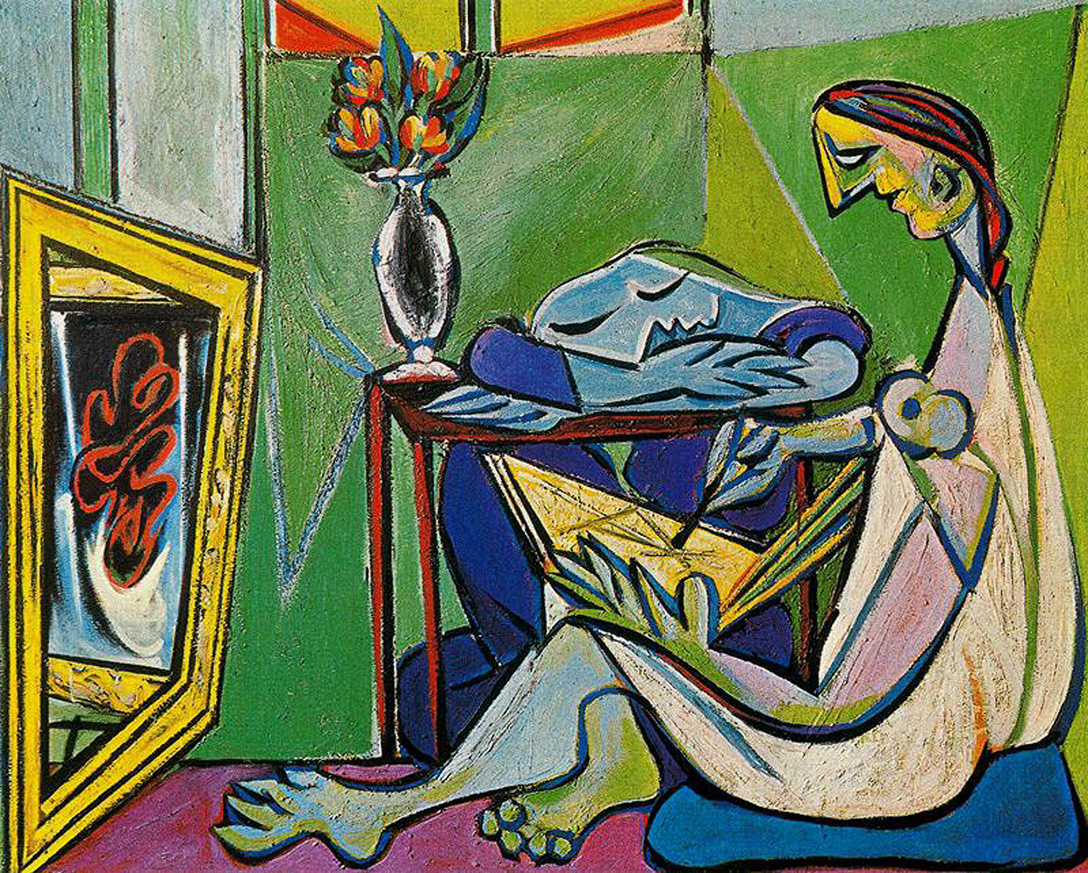
\includegraphics[height=2.5cm, width=0.7\textwidth]{style6}
        \label{fig:anaoas_style6}
        \caption{The Muse, Pablo Picasso, 1935}
	\end{subfigure}
    \hfill
    \begin{subfigure}[b]{0.4\textwidth}
		\centering
        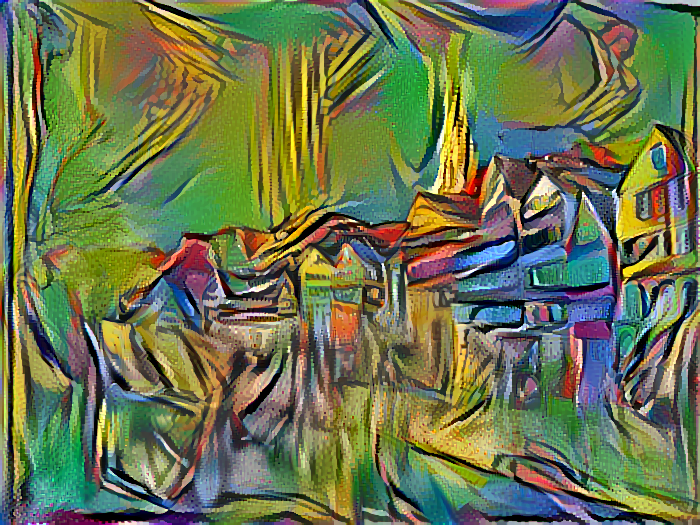
\includegraphics[height=4cm, width=1.1\textwidth]{anaoas_c1s6}
        \label{fig:anaoas_c1s6}
	\end{subfigure}
    \begin{subfigure}[b]{0.5\textwidth}
		\centering
        \includegraphics[height=2.5cm, width=0.7\textwidth]{style7}
        \label{fig:anaoas_style7}
        \caption{The Great Wave off Kanagawa, Hokusai, 1829-1832}
	\end{subfigure}
    \hfill
    \begin{subfigure}[b]{0.4\textwidth}
		\centering
        \includegraphics[height=4cm, width=1.1\textwidth]{anaoas_c1s7}
        \label{fig:anaoas_c1s7}
	\end{subfigure}
\end{figure}

\begin{figure}[H]
	\centering
    \begin{subfigure}[b]{0.19\textwidth}
		\centering
        \includegraphics[height=2.5cm, width=1\textwidth]{style1}
        \label{fig:anaoas_style1}
	\end{subfigure}
    \hfill
    \begin{subfigure}[b]{0.19\textwidth}
		\centering
        \includegraphics[height=2.5cm, width=1\textwidth]{content2}
        \label{fig:anaoas_conten2}
	\end{subfigure}
    \hfill
    \begin{subfigure}[b]{0.19\textwidth}
		\centering
        \includegraphics[height=2.5cm, width=1\textwidth]{anaoas_c2s1}
        \label{fig:anaoas_c2s1}
	\end{subfigure}
    \hfill
    \begin{subfigure}[b]{0.19\textwidth}
		\centering
        \includegraphics[height=2.5cm, width=1\textwidth]{content3}
        \label{fig:anaoas_conten3}
	\end{subfigure}
    \hfill
    \begin{subfigure}[b]{0.19\textwidth}
		\centering
        \includegraphics[height=2.5cm, width=1\textwidth]{anaoas_c3s1}
        \label{fig:anaoas_c3s1}
	\end{subfigure}
    \begin{subfigure}[b]{0.19\textwidth}
		\centering
        \includegraphics[height=2.5cm, width=1\textwidth]{style2}
        \label{fig:anaoas_style2}
	\end{subfigure}
    \hfill
    \begin{subfigure}[b]{0.19\textwidth}
		\centering
        \includegraphics[height=2.5cm, width=1\textwidth]{content2}
        \label{fig:anaoas_conten2}
	\end{subfigure}
    \hfill
    \begin{subfigure}[b]{0.19\textwidth}
		\centering
        \includegraphics[height=2.5cm, width=1\textwidth]{anaoas_c2s2}
        \label{fig:anaoas_c2s2}
	\end{subfigure}
    \hfill
    \begin{subfigure}[b]{0.19\textwidth}
		\centering
        \includegraphics[height=2.5cm, width=1\textwidth]{content3}
        \label{fig:anaoas_conten3}
	\end{subfigure}
    \hfill
    \begin{subfigure}[b]{0.19\textwidth}
		\centering
        \includegraphics[height=2.5cm, width=1\textwidth]{anaoas_c3s2}
        \label{fig:anaoas_c3s2}
	\end{subfigure}
    \begin{subfigure}[b]{0.19\textwidth}
		\centering
        \includegraphics[height=2.5cm, width=1\textwidth]{style3}
        \label{fig:anaoas_style3}
	\end{subfigure}
    \hfill
    \begin{subfigure}[b]{0.19\textwidth}
		\centering
        \includegraphics[height=2.5cm, width=1\textwidth]{content2}
        \label{fig:anaoas_conten2}
	\end{subfigure}
    \hfill
    \begin{subfigure}[b]{0.19\textwidth}
		\centering
        \includegraphics[height=2.5cm, width=1\textwidth]{anaoas_c2s3}
        \label{fig:anaoas_c2s3}
	\end{subfigure}
    \hfill
    \begin{subfigure}[b]{0.19\textwidth}
		\centering
        \includegraphics[height=2.5cm, width=1\textwidth]{content3}
        \label{fig:anaoas_conten3}
	\end{subfigure}
    \hfill
    \begin{subfigure}[b]{0.19\textwidth}
		\centering
        \includegraphics[height=2.5cm, width=1\textwidth]{anaoas_c3s3}
        \label{fig:anaoas_c3s3}
	\end{subfigure}
    \begin{subfigure}[b]{0.19\textwidth}
		\centering
        \includegraphics[height=2.5cm, width=1\textwidth]{style4}
        \label{fig:anaoas_style4}
	\end{subfigure}
    \hfill
    \begin{subfigure}[b]{0.19\textwidth}
		\centering
        \includegraphics[height=2.5cm, width=1\textwidth]{content2}
        \label{fig:anaoas_conten2}
	\end{subfigure}
    \hfill
    \begin{subfigure}[b]{0.19\textwidth}
		\centering
        \includegraphics[height=2.5cm, width=1\textwidth]{anaoas_c2s4}
        \label{fig:anaoas_c2s4}
	\end{subfigure}
    \hfill
    \begin{subfigure}[b]{0.19\textwidth}
		\centering
        \includegraphics[height=2.5cm, width=1\textwidth]{content3}
        \label{fig:anaoas_conten3}
	\end{subfigure}
    \hfill
    \begin{subfigure}[b]{0.19\textwidth}
		\centering
        \includegraphics[height=2.5cm, width=1\textwidth]{anaoas_c3s4}
        \label{fig:anaoas_c3s4}
	\end{subfigure}
    \begin{subfigure}[b]{0.19\textwidth}
		\centering
        \includegraphics[height=2.5cm, width=1\textwidth]{style5}
        \label{fig:anaoas_style5}
	\end{subfigure}
    \hfill
    \begin{subfigure}[b]{0.19\textwidth}
		\centering
        \includegraphics[height=2.5cm, width=1\textwidth]{content2}
        \label{fig:anaoas_conten2}
	\end{subfigure}
    \hfill
    \begin{subfigure}[b]{0.19\textwidth}
		\centering
        \includegraphics[height=2.5cm, width=1\textwidth]{anaoas_c2s5}
        \label{fig:anaoas_c2s5}
	\end{subfigure}
    \hfill
    \begin{subfigure}[b]{0.19\textwidth}
		\centering
        \includegraphics[height=2.5cm, width=1\textwidth]{content3}
        \label{fig:anaoas_conten3}
	\end{subfigure}
    \hfill
    \begin{subfigure}[b]{0.19\textwidth}
		\centering
        \includegraphics[height=2.5cm, width=1\textwidth]{anaoas_c3s5}
        \label{fig:anaoas_c3s5}
	\end{subfigure}
    \begin{subfigure}[b]{0.19\textwidth}
		\centering
        \includegraphics[height=2.5cm, width=1\textwidth]{style6}
        \label{fig:anaoas_style6}
	\end{subfigure}
    \hfill
    \begin{subfigure}[b]{0.19\textwidth}
		\centering
        \includegraphics[height=2.5cm, width=1\textwidth]{content2}
        \label{fig:anaoas_conten2}
	\end{subfigure}
    \hfill
    \begin{subfigure}[b]{0.19\textwidth}
		\centering
        \includegraphics[height=2.5cm, width=1\textwidth]{anaoas_c2s6}
        \label{fig:anaoas_c2s6}
	\end{subfigure}
    \hfill
    \begin{subfigure}[b]{0.19\textwidth}
		\centering
        \includegraphics[height=2.5cm, width=1\textwidth]{content3}
        \label{fig:anaoas_conten3}
	\end{subfigure}
    \hfill
    \begin{subfigure}[b]{0.19\textwidth}
		\centering
        \includegraphics[height=2.5cm, width=1\textwidth]{anaoas_c3s6}
        \label{fig:anaoas_c3s6}
	\end{subfigure}
    \begin{subfigure}[b]{0.19\textwidth}
		\centering
        \includegraphics[height=2.5cm, width=1\textwidth]{style7}
        \label{fig:anaoas_style7}
	\end{subfigure}
    \hfill
    \begin{subfigure}[b]{0.19\textwidth}
		\centering
        \includegraphics[height=2.5cm, width=1\textwidth]{content2}
        \label{fig:anaoas_conten2}
	\end{subfigure}
    \hfill
    \begin{subfigure}[b]{0.19\textwidth}
		\centering
        \includegraphics[height=2.5cm, width=1\textwidth]{anaoas_c2s7}
        \label{fig:anaoas_c2s7}
	\end{subfigure}
    \hfill
    \begin{subfigure}[b]{0.19\textwidth}
		\centering
        \includegraphics[height=2.5cm, width=1\textwidth]{content3}
        \label{fig:anaoas_conten3}
	\end{subfigure}
    \hfill
    \begin{subfigure}[b]{0.19\textwidth}
		\centering
        \includegraphics[height=2.5cm, width=1\textwidth]{anaoas_c3s7}
        \label{fig:anaoas_c3s7}
	\end{subfigure}
    \caption{}
    \label{fig:anaoas_diverse_rezultate}
\end{figure}

\begin{figure}[h]
	\centering
    \begin{subfigure}[b]{0.19\textwidth}
		\centering
        \includegraphics[height=2.8cm, width=1\textwidth]{style1}
        \label{fig:anaoas_style1}
        \caption{}
	\end{subfigure}
    \hfill
    \begin{subfigure}[b]{0.19\textwidth}
		\centering
        \includegraphics[height=2.8cm, width=1\textwidth]{content1}
        \label{fig:anaoas_conten1}
        \caption{}
	\end{subfigure}
    \hfill
    \begin{subfigure}[b]{0.19\textwidth}
		\centering
        \includegraphics[height=2.8cm, width=1\textwidth]{anaoas_c1s1}
        \label{fig:anaoas_c1s1}
        \caption{}
	\end{subfigure}
    \hfill
    \begin{subfigure}[b]{0.19\textwidth}
		\centering
        \includegraphics[height=2.8cm, width=1\textwidth]{anaoas_c1s1_stil400}
        \label{fig:anaoas_c1s1_stil400}
        \caption{}
	\end{subfigure}
    \hfill
    \begin{subfigure}[b]{0.19\textwidth}
		\centering
        \includegraphics[height=2.8cm, width=1\textwidth]{anaoas_c1s1_stil1400}
        \label{fig:anaoas_c1s1_stil1400}
        \caption{}
	\end{subfigure}
    \caption{În această figură se observă impactul pe care îl are poza cu stil la diferite dimensiuni. Poza $(b)$ a avut dimensiunea $max(lungime, latime) = 700$ de pixeli. Pentru generarea pozei $(c)$, poza $(a)$ a avut dimensiunea $max(lungime, latime) = 700$ de pixeli. Pentru generarea pozei $(d)$, poza $(a)$ a avut dimensiunea $max(lungime, latime) = 400$ de pixeli. Pentru generarea pozei $(e)$, poza $(a)$ a avut dimensiunea $max(lungime, latime) = 1400$ de pixeli.}
\end{figure}

Pozele cu conținut din figura [\ref{fig:anaoas_diverse_rezultate}] au fost luate de pe github-ul lui Justin Johnson \cite{continut_chicago}, respectiv \cite{continut_hoover_tower}.

În poza [\ref{fig:tradeoff}] se poate observa compromisul dintre conținut și stil. Pentru stil, pentru pozele de pe linia $A$ am folosit activările din layerul \textit{conv1{\_}1}, pentru pozele de pe linia $B$ am folosit layerele \textit{conv1{\_}1} și \textit{conv2{\_}1}, pentru pozele de pe linia $C$ am folosit layerele \textit{conv1{\_}1}, \textit{conv2{\_}1} și \textit{conv3{\_}1}, pentru pozele de pe linia $D$ am folosit layerele \textit{conv1{\_}1}, \textit{conv2{\_}1}, \textit{conv3{\_}1} și \textit{conv4{\_}1}, iar pentru pozele de pe linia $E$ am folosit layerele \textit{conv1{\_}1}, \textit{conv2{\_}1}, \textit{conv3{\_}1}, \textit{conv4{\_}1} și \textit{conv5{\_}1}. Iar pentru conținut, pentru toate pozele am folosit activările din layerul \textit{conv4{\_}2}.

\begin{figure}[h]
	\centering
    \begin{subfigure}[b]{0.3\textwidth}
    	A
		\centering
        \includegraphics[height=4cm, width=0.9\textwidth]{anaoas_ratio2_11}
        \label{anaoas_ratio2_11}
	\end{subfigure}
    \hfill
    \begin{subfigure}[b]{0.3\textwidth}
		\centering
        \includegraphics[height=4cm, width=0.9\textwidth]{anaoas_ratio1_11}
        \label{fig:anaoas_ratio1_11}
	\end{subfigure}
    \hfill
    \begin{subfigure}[b]{0.3\textwidth}
		\centering
        \includegraphics[height=4cm, width=0.9\textwidth]{anaoas_ratio3_11}
        \label{fig:anaoas_ratio3_11}
	\end{subfigure}
    \begin{subfigure}[b]{0.3\textwidth}
    	B
		\centering
        \includegraphics[height=4cm, width=0.9\textwidth]{anaoas_ratio2_21}
        \label{fig:anaoas_ratio2_21}
	\end{subfigure}
    \hfill
    \begin{subfigure}[b]{0.3\textwidth}
		\centering
        \includegraphics[height=4cm, width=0.9\textwidth]{anaoas_ratio1_21}
        \label{fig:anaoas_ratio1_21}
	\end{subfigure}
    \hfill
    \begin{subfigure}[b]{0.3\textwidth}
		\centering
        \includegraphics[height=4cm, width=0.9\textwidth]{anaoas_ratio3_21}
        \label{fig:anaoas_ratio3_21}
	\end{subfigure}
    \begin{subfigure}[b]{0.3\textwidth}
    	C
		\centering
        \includegraphics[height=4cm, width=0.9\textwidth]{anaoas_ratio2_31}
        \label{fig:anaoas_ratio2_31}
	\end{subfigure}
    \hfill
    \begin{subfigure}[b]{0.3\textwidth}
		\centering
        \includegraphics[height=4cm, width=0.9\textwidth]{anaoas_ratio1_31}
        \label{fig:anaoas_ratio1_31}
	\end{subfigure}
    \hfill
    \begin{subfigure}[b]{0.3\textwidth}
		\centering
        \includegraphics[height=4cm, width=0.9\textwidth]{anaoas_ratio3_31}
        \label{fig:anaoas_ratio3_31}
	\end{subfigure}
    \begin{subfigure}[b]{0.3\textwidth}
    	D
		\centering
        \includegraphics[height=4cm, width=0.9\textwidth]{anaoas_ratio2_41}
        \label{fig:anaoas_ratio2_41}
	\end{subfigure}
    \hfill
    \begin{subfigure}[b]{0.3\textwidth}
		\centering
        \includegraphics[height=4cm, width=0.9\textwidth]{anaoas_ratio1_41}
        \label{fig:anaoas_ratio1_41}
	\end{subfigure}
    \hfill
    \begin{subfigure}[b]{0.3\textwidth}
		\centering
        \includegraphics[height=4cm, width=0.9\textwidth]{anaoas_ratio3_41}
        \label{fig:anaoas_ratio3_41}
	\end{subfigure}
    \begin{subfigure}[b]{0.3\textwidth}
    	E
		\centering
        \includegraphics[height=4cm, width=0.9\textwidth]{anaoas_ratio2_51}
        \caption{$\alpha = 100$, $\beta = 10$, $\gamma = 0$}
        \label{fig:anaoas_ratio2_51}
	\end{subfigure}
    \hfill
    \begin{subfigure}[b]{0.3\textwidth}
		\centering
        \includegraphics[height=4cm, width=0.9\textwidth]{anaoas_ratio1_51}
        \caption{$\alpha = 100$, $\beta = 1$, $\gamma = 0$}
        \label{fig:anaoas_ratio2_51}
	\end{subfigure}
    \hfill
    \begin{subfigure}[b]{0.3\textwidth}
		\centering
        \includegraphics[height=4cm, width=0.9\textwidth]{anaoas_ratio3_51}
        \caption{$\alpha = 1000$, $\beta = 1$, $\gamma = 0$}
        \label{fig:anaoas_ratio3_51}
	\end{subfigure}
    \caption{}
    \label{fig:tradeoff}
\end{figure}

\chapter{Transferul stilului artistic fotografic}\thispagestyle{fancy}
\label{dpst}
\section{Introducere}
După cum am văzut în capitolul Un algoritm neural al stilului artistic [\ref{anaoas}] este posibil ca stilul și conținutul unei poze să fie separabile, și astfel combinând două poze oarecare să se obțină o poză nouă care combină conținutul uneia dintre poze cu stilul celeilalte.

Deși această metodă oferă rezultate satisfăcătoare, se pune problema ca poza obținută să fie cât mai fotografică. Chiar dacă folosim metoda lui Leon A. Gatys pe două poze care sunt fotografice, de exemplu două poze făcute unor blocuri dintr-un oraș, atunci tot apar nereguli în poza generată, lucru pe care nu ni l-am dori, am dori ca poza generată să fie tot una fotografică. Am vrea să se păstreze conținutul semantic în timpul combinării conținutului cu stilul. De exemplu dacă în poza cu stil se vede cerul, atunci este posibil ca în poza generată, părți ale cerului să apară pe unele obiecte din poza cu conținut deoarece, formula [\ref{eq:style_loss}] nu ține cont de unde apare respectivul stil în imagine, ci doar că acesta trebuie să fie prezent în locuri aleatoare. Pentru a rezolva această problemă este nevoie de o constrângere pentru formula [\ref{eq:style_loss}] pentru a forța algoritmul să respecte conținutul semantic. În articolul său \cite{luan2017} Fujun Luan propune introducerea de măști pentru poza de conținut și poza de stil. Aceste măști etichetează obiectele cu același înțeles semantic din cele două poze, atribuindu-le o etichetă.

În cele ce urmează o să dovedesc că această îmbunătățire adusă de Fujun Luan algoritmului lui Leon A. Gatys este fiabilă în generarea de poze fotografice venind cu mai multe exemple. De asemenea, o altă aplicabilitate pe care o aduc măștile pentru pozele de conținut și stil este aceea că de exemplu, putem modifica culoarea unor obiecte din aceeași poză între ele.

\subsection{Etichetări semantice}
\label{semantic_segmentation}
Pentru cazul descris mai sus, cel în care ne dorim să păstrăm conținutul semantic atunci când combinăm conținutul cu stilul a două poze, voi prezenta soluția lui Fujun Luan, aceea de a introduce măști cu ajutorul cărora putem eticheta obiectele cu același înțeles semantic. Pe lângă faptul că aceste măști impun algoritmului să aducă modificări doar obiectelor asemănătoare, mai oferă și posibilitatea utilizatorului de a transfera stilul doar acelor obiecte de care este interesat și astfel obținând noi poze aparte.

\section{Metodă}
În această secțiune voi defini o funcție de cost, asemănătoare cu cea din capitolul [\ref{anaoas}] [\ref{eq:total_loss}], propusă de Fujun Luan în articolul său.

Pentru notații, le vom folosi tot pe cele definite anterior, la care o să mai adăugam unele noi.

Funcția de cost pentru conținut este aceeași cu cea definită la [\ref{eq:content_loss}].

Reamintesc că funcția de cost pentru stil este definită la [\ref{eq:style_loss}]. Pentru a rezolva problema enunțată în [\ref{semantic_segmentation}] vom modifica această funcție de cost pentru a constrânge algoritmul să aplice un anumit stil doar pe porțiunile cu același înțeles semantic din poza de conținut și poza de stil cu ajutorul măștilor. Fie $M_{l, c}$ masca pentru o poză din layerul $l$ și $c$ canalul măștii respective pentru acel layer. Pentru pozele $\vec{x}$ și $\vec{s}$ considerăm matricele $XM_{l, c}$, respectiv $SM_{l, c}$. Atunci înmulțind matricele $XV^l \in \mathcal{R}^{N^{l} \times M^{l}}$ și $SV^l \in \mathcal{R}^{N^{l} \times M^{l}}$ cu matricele măștilor obținem $XV^{l, c} = XV^l XM_{l, c}$, respectiv $SV^{l, c} = SV^l SM_{l, c}$. Astfel, matricele gram devin $XG_{ij}^{l, c} = \displaystyle \sum_{k}{XV_{ik}^{l, c} XV_{jk}^{l, c}}$, respectiv $SG_{ij}^{l, c} = \displaystyle \sum_{k}{SV_{ik}^{l, c} SV_{jk}^{l, c}}$ și costul dintr-un anumit layer devine:
\begin{equation}
\label{eq:layer_style_loss_dpst}
E_l = \sum_{c=1}^{C}{\frac{1}{4(H^{l})^{2}(W^{l})^{2}(C^{l})^{2}} \sum_{i, j}{(SG_{ij}^{l, c} - XG_{ij}^{l, c})^2}}
\end{equation}
unde $C$ este numărul total de canale din mască.

Atunci, funcția de cost pentru stil este definită astfel:
\begin{equation}
\label{eq:style_loss_dpst}
\mathcal{L}_{stil+}(\vec{s}, \vec{x}) = \sum_{l=1}^{L} w_l E_l
\end{equation}

Astfel, având definite toate costurile intermediare, putem defini costul total:
\begin{equation}
\label{eq:total_loss_dpst}
\mathcal{L}_{total}(\vec{c}, \vec{s}, \vec{x}) = \alpha \mathcal{L}_{continut}(\vec{c}, \vec{x}) + \beta \mathcal{L}_{stil}(\vec{s}, \vec{x}) + \gamma \mathcal{L}_{zgomot}(\vec{x})
\end{equation}
unde parametrii $\alpha$, $\beta$ și $\gamma$ controlează compromisul dintre conținut, stil și zgomot, iar $\mathcal{L}_{zgomot}(\vec{x})$ este funcția de cost definită în [\ref{eq:tv_loss}].

\section{Detalii de implementare}
Pentru a implementa metoda de mai sus am folosit același procedeu descris în capitolul Un algoritm neural al stilului artistic [\ref{anaoas}] cu o mică adăugare. Și anume, după ce am trecut imaginile prin rețeaua VGG19, am adăugat măștile peste activările din layerele respective și am fost atent ca atunci când am aplicat masca pe activările din layerele pentru stil, aceasta să fie de aceeași dimensiune cu matricea activărilor, deoarece imaginea este micșorată de-a lungul rețelei.

Și pentru această metodă am folosit aceeași parametri ca cei menționați în capitolul precedent.

Măștile pentru poze le-am creat manual în programul de editare de imagini numit GIMP. Această abordare de creare manuală a măștilor oferă o arie mai largă de generare de poze artistice, cel care folosește acest algoritm, fiind liber să aleagă între ce obiecte din poză să fie făcut transferul de stil. Culorile prezente în măștile pe care le-am folosit pentru acest algoritm sunt alb, negru, roșu, verde sau albastru, numărul acestora fiind suficient pentru păstrarea înțelesului semantic în pozele pe care le-am întâlnit. De asemenea, se mai pot adăuga oricâte culori dacă pozele sunt complexe și există multe obiecte diferite. În cazul în care nu se dorește transferul stilului pentru un anumit obiect, atunci în mască, pentru acel obiect trebuie să fie o culoare care nu este prezentă în cele definite, eu am folosit culoarea gri pentru acest caz. Un lucru la care a trebuit să mai fiu atent când am creat măștile este acela să nu am obiecte marcate în masca pentru poza de conținut, dar care nu sunt prezente în masca pentru poza de stil sau invers, deoarece algoritmul nu ar mai funcționa cum trebuie, neavând între ce obiecte să facă transferul de stil.

\newpage
\section{Rezultate și comparații}
Toate pozele cu stil și cu conținut sunt luate din articolul lui Fujun Luan, Deep Photo Style Transfer \cite{luan2017}.
\begin{figure}[h]
	\centering
    \begin{subfigure}[b]{0.49\textwidth}
		\centering
        \includegraphics[height=5.2cm, width=1.01\textwidth]{d_content1}
        \label{fig:dpst_d_content1}
        \caption{Poza cu conținut}
	\end{subfigure}
    \hfill
    \begin{subfigure}[b]{0.49\textwidth}
		\centering
        \includegraphics[height=5.2cm, width=1.01\textwidth]{d_style1}
        \label{fig:dpst_d_style1}
        \caption{Poza cu stil}
	\end{subfigure}
    \begin{subfigure}[b]{0.49\textwidth}
		\centering
        \includegraphics[height=5.2cm, width=1.01\textwidth]{dpst_c1s1_luan}
        \label{fig:dpst_c1s1_luan}
        \caption{Poză luată din articolul lui Fujun Luan}
	\end{subfigure}
    \hfill
    \begin{subfigure}[b]{0.49\textwidth}
		\centering
        \includegraphics[height=5.2cm, width=1.01\textwidth]{dpst_c1s1}
        \label{fig:dpst_c1s1}
        \caption{Poză generată de mine}
	\end{subfigure}
    \caption{Cele două poze sunt diferite, deoarece în poza din stânga, autorul mai aplică unele optimizări în plus. De asemenea, mai intră în calcul și dimensiunea pozelor cu conținut și stil care au fost folosite la generarea celei de-a treia poze.}
\end{figure}

În continuare, voi mai prezenta și alte rezultate pentru a exemplifica posibilitățile pe care le oferă această metoda, cum ar fi schimbarea anotimpului dintr-o poză sau modificarea doar a anumitor obiecte din poză folosind măștile.

\begin{figure}[h]
	\centering
    \begin{subfigure}[b]{0.3\textwidth}
		\centering
        \includegraphics[height=4.7cm, width=1.01\textwidth]{d_content2}
        \label{fig:dpst_d_content2}
	\end{subfigure}
    \hfill
    \begin{subfigure}[b]{0.3\textwidth}
		\centering
        \includegraphics[height=4.7cm, width=1.01\textwidth]{d_style2}
        \label{fig:dpst_d_style2}
	\end{subfigure}
    \hfill
    \begin{subfigure}[b]{0.3\textwidth}
		\centering
        \includegraphics[height=4.7cm, width=1.01\textwidth]{dpst_c2s2}
        \label{fig:dpst_c2s2}
	\end{subfigure}
    \begin{subfigure}[b]{0.3\textwidth}
		\centering
        \includegraphics[height=4.7cm, width=1.01\textwidth]{d_content5}
        \label{fig:dpst_d_content5}
	\end{subfigure}
    \hfill
    \begin{subfigure}[b]{0.3\textwidth}
		\centering
        \includegraphics[height=4.7cm, width=1.01\textwidth]{d_style5}
        \label{fig:dpst_d_style5}
	\end{subfigure}
    \hfill
    \begin{subfigure}[b]{0.3\textwidth}
		\centering
        \includegraphics[height=4.7cm, width=1.01\textwidth]{dpst_c5s5}
        \label{fig:dpst_c5s5}
	\end{subfigure}
    \caption{}
\end{figure}

\begin{figure}[h]
	\centering
    \begin{subfigure}[b]{0.3\textwidth}
		\centering
        \includegraphics[height=4.7cm, width=1.01\textwidth]{d_content4}
        \label{fig:dpst_d_content4}
	\end{subfigure}
    \hfill
    \begin{subfigure}[b]{0.3\textwidth}
		\centering
        \includegraphics[height=4.7cm, width=1.01\textwidth]{d_style4}
        \label{fig:dpst_d_style4}
	\end{subfigure}
    \hfill
    \begin{subfigure}[b]{0.3\textwidth}
		\centering
        \includegraphics[height=4.7cm, width=1.01\textwidth]{dpst_c4s4}
        \label{fig:dpst_c4s4}
	\end{subfigure}
    \begin{subfigure}[b]{0.3\textwidth}
		\centering
        \includegraphics[height=4.7cm, width=1.01\textwidth]{d_content7}
        \label{fig:dpst_d_content7}
	\end{subfigure}
    \hfill
    \begin{subfigure}[b]{0.3\textwidth}
		\centering
        \includegraphics[height=4.7cm, width=1.01\textwidth]{d_style7}
        \label{fig:dpst_d_style7}
	\end{subfigure}
    \hfill
    \begin{subfigure}[b]{0.3\textwidth}
		\centering
        \includegraphics[height=4.7cm, width=1.01\textwidth]{dpst_c7s7}
        \label{fig:dpst_c7s7}
	\end{subfigure}
    \caption{Poze mai puțin reușite din cauza complexității și din cauza nepotrivirii intocmai a conținutului cu stilul.}
\end{figure}

\begin{figure}[h]
	\centering
    \begin{subfigure}[b]{0.24\textwidth}
		\centering
        \includegraphics[height=3.5cm, width=1.01\textwidth]{d_content6}
        \label{fig:dpst_d_content6}
	\end{subfigure}
    \hfill
    \begin{subfigure}[b]{0.24\textwidth}
		\centering
        \includegraphics[height=3.5cm, width=1.01\textwidth]{mask_d_content6}
        \label{fig:dpst_d_mask_content6}
	\end{subfigure}
    \hfill
    \begin{subfigure}[b]{0.24\textwidth}
		\centering
        \includegraphics[height=3.5cm, width=1.01\textwidth]{mask_d_style6}
        \label{fig:dpst_d_mask_style6}
	\end{subfigure}
    \hfill
    \begin{subfigure}[b]{0.24\textwidth}
		\centering
        \includegraphics[height=3.5cm, width=1.01\textwidth]{dpst_c6s6}
        \label{fig:dpst_c6s6}
	\end{subfigure}
    \caption{În această figură se poate vedea avantajul măștii. Poza din stânga este tratată și ca poză de conținut și ca poză de stil. Poza a doua reprezintă masca pentru poza care este generată, iar a treia poză reprezintă masca pentru poza cu stil. Ultima poză este poza generată de către algoritm.}
\end{figure}

\begin{figure}[h]
	\centering
    \begin{subfigure}[b]{0.24\textwidth}
		\centering
        \includegraphics[height=4cm, width=1.01\textwidth]{d_content3}
        \label{fig:dpst_d_content3}
	\end{subfigure}
    \hfill
    \begin{subfigure}[b]{0.24\textwidth}
		\centering
        \includegraphics[height=4cm, width=1.01\textwidth]{d_style3}
        \label{fig:dpst_d_style3}
	\end{subfigure}
    \hfill
    \begin{subfigure}[b]{0.24\textwidth}
		\centering
        \includegraphics[height=4cm, width=1.01\textwidth]{dpst_c3s3}
        \label{fig:dpst_d_mask_style3}
	\end{subfigure}
    \hfill
    \begin{subfigure}[b]{0.24\textwidth}
		\centering
        \includegraphics[height=4cm, width=1.01\textwidth]{dpst_c3s3_content}
        \label{fig:dpst_c3s3_content}
	\end{subfigure}
    \caption{În această figură, pentru generarea pozei a treia am pornit de la o poză inițializată cu zgomot, iar pentru generarea ultimei poze, am pornit de la o poză inițializată cu poza de conținut peste care am adăugat zgomot aleator. Se poate observa că folosind ultima metodă algoritmul învață mai ușor reprezentarea conținutului, iar stilul are un impact mai scăzut.}
\end{figure}

\begin{figure}[h]
	\centering
    \begin{subfigure}[b]{0.24\textwidth}
		\centering
        \includegraphics[height=4cm, width=1.01\textwidth]{dpst_c1s1_lambda0_001}
        \label{fig:dpst_c1s1_lambda0_001}
        \caption{$\gamma = 0.001$}
	\end{subfigure}
    \hfill
    \begin{subfigure}[b]{0.24\textwidth}
		\centering
        \includegraphics[height=4cm, width=1.01\textwidth]{dpst_c1s1_lambda0_01}
        \label{fig:dpst_c1s1_lambda0_01}
        \caption{$\gamma = 0.01$}
	\end{subfigure}
    \hfill
    \begin{subfigure}[b]{0.24\textwidth}
		\centering
        \includegraphics[height=4cm, width=1.01\textwidth]{dpst_c1s1_lambda0_1}
        \label{fig:dpst_c1s1_lambda0_1}
        \caption{$\gamma = 0.1$}
	\end{subfigure}
    \hfill
    \begin{subfigure}[b]{0.24\textwidth}
		\centering
        \includegraphics[height=4cm, width=1.01\textwidth]{dpst_c1s1_lambda1}
        \label{fig:dpst_c1s1_lambda1}
        \caption{$\gamma = 1$}
	\end{subfigure}
    \caption{În această figură se poate vedea impactul pe care îl are $\gamma$, parametrul care controlează importanța funcției de cost pentru zgomot.}
\end{figure}

\chapter{Transferul stilului artistic în timp real}\thispagestyle{fancy}
\label{plfrtst}
\section{Introducere}
Deși metodele prezentate în capitolele [\ref{anaoas}] și [\ref{dpst}] demonstrează faptul că se pot obține poze artistice combinând conținutul și stilul a două poze, timpul necesar pentru generarea unei astfel de poze este unul destul de mare. În acest capitol voi prezenta o soluție la problema de mai sus descrisă de Justin Johnson în articolul său \cite{johnson2016}. După cum știm, se poate antrena o rețea neurală convoluțională pentru a rezolva diferite probleme care conțin imagini, precum recunoașterea de obiecte sau segmentarea obiectelor dintr-o poză. Plecând de la această idee și folosind metoda lui Leon A. Gatys de separare a stilului și conținutului, Justin Johnson propune antrenarea unei rețele neurale convoluționale pentru a învăța să aplice un anumit stil pe o poză.

În cele ce urmează voi arăta că soluția lui Justin Johnson este una fiabilă, obținând rezultate asemănătoare cu cele date de algoritmul lui Leon A. Gatys. Pe lângă faptul acesta, timpul de generare a unei poze artistice este redus semnificativ, deoarece este nevoie doar de o parcurgere a pozei inițiale prin rețea, singura parte care necesită un timp mai mare fiind aceea de antrenare a rețelei.

\section{Metodă}
Pentru a putea antrena o rețea neurală convoluțională care să învețe să aplice un anumit stil pe poze este nevoie să ne definim o funcție de cost. Ne vom folosi de funcțiile de cost prezentate în capitolul Un algoritm neural al stilului artistic [\ref{anaoas}]. Și anume, funcția de cost pentru conținut este cea definită la [\ref{eq:content_loss}], funcția de cost pentru stil este cea definită la [\ref{eq:style_loss}], funcția de zgomot pentru poza care urmează să fie generată este cea definită la [\ref{eq:tv_loss}] și funcția de cost finală este cea de la [\ref{eq:total_loss}].

\section{Detalii de implementare}
Deoarece această metodă este diferită de cele doua prezentate anterior, procedeul pe care l-am urmat pentru a implementa-o este diferit. În primul rând este necesar să antrenez o rețea neurală convoluțională care să învețe să aplice un anumit stil. Așadar am folosit rețeaua propusă de Justin Johnson în articolul său, pe care a numit-o Transform Net. Arhitectura acestei rețele se poate observa în imaginea [\ref{fig:transform_net_arh}]. În această imagine, $C$ $x$ $H$ $x$ $W$ $conv$ este interpretat astfel: $C$ este numărul de filtre din layer, $H$ este lungimea filtrului, iar $W$ este lățimea filtrului. $Stride$ $n$ este numărul de pixeli pe care să îl sară filtrul atunci când este plimbat pe imagine. De asemenea se observă că apar și 5 blocuri reziduale [\ref{fig:res_block}]. După fiecare layer non-rezidual este aplicată o normalizare a batch-ului [\ref{sb:batch_norm}] urmată de funcția de activare ReLU, mai puțin pentru ultimul layer, unde în loc de ReLU este folosită funcția de activare tanh (tangenta hiperbolică) [\ref{sb:tanh}] pentru că ne dorim ca pixelii pozei întoarse de rețea să fie între $[-1, 1]$. Arhitectura acestei rețele este una interesantă deoarece inițial, rețeaua reduce dimensiunea pozei de intrare până la un anumit punct pentru a putea învăța caracteristici mai complexe, apoi la această dimensiune sunt aplicate o serie de blocuri reziduale, iar mai apoi imaginea este mărită cu ajutorul layerelor ce poartă numele de layere convoluționale transpuse ajungând la dimensiunea inițială.

La fel ca și la metoda lui Leon A. Gatys, algoritmul primește ca date de intrare două poze, una cu conținutul dorit și una cu stilul. La acest algoritm nu mai este nevoie să fie inițializată cu zgomot aleator o a treia poză deoarece este folosită rețeaua să învețe aplicarea stilului respectiv. Așadar, poza de conținut am normalizat-o și am trecut-o prin rețeaua Transform Net obținând o imagine nouă. Apoi am trecut cele trei poze, poza obținută de la Transform Net, poza cu conținutul și poza cu stilul prin rețeaua VGG19, și la fel ca la metoda lui Leon A. Gatys, am salvat activările din layerul \textit{conv4{\_}2} pentru conținut și activările din layerele \textit{conv1{\_}1}, \textit{conv2{\_}1}, \textit{conv3{\_}1}, \textit{conv4{\_}1}, \textit{conv5{\_}1} pentru stil pentru a putea calcula funcțiile de cost. Pe baza acestor funcții de cost, cu ajutorul algoritmului de coborâre pe gradient și a metodei backpropagation am optimizat valorile filtrelor pentru a obține un cost total cât mai mic.

În imaginea \ref{fig:transform_vgg_workflow} se poate observa procesul pe care l-am descris mai sus.

\begin{figure}[H]
		\centering
        \includegraphics[width=\textwidth]{transform_vgg_workflow}
        \caption{Workflow-ul algoritmului}
        \label{fig:transform_vgg_workflow}
\end{figure}

Pentru a învăța aplicarea unui anumit stil, rețeaua Transform Net are nevoie de multe poze cu conținut. De aceea, pentru antrenare, am folosit setul de date Microsoft COCO [\ref{sb:microsoft_coco}]. Setul de antrenare conține aproximativ $80000$ de poze. Pentru rezultatele din această lucrare am antrenat rețeaua timp de $10000$ de iterații, fiecare iterație conținând un batch de 4 poze luate aleator din setul de antrenare pe care le-am redimensionat la dimensiunea de $256$ $x$ $256$ pixeli. De asemenea și poza cu conținut și poza cu stil le-am redimensionat la $256$ $x$ $256$ de pixeli. Antrenarea a durat aproximativ 7 ore pe Google Cloud, pe o placă video NVIDIA Tesla K80.

Parametrii folosiți în timpul antrenării au fost $\alpha = 1000$, $\beta = 1$ și rata de învățare egală cu 0.001.

\begin{figure}[h]
	\centering
    \begin{subfigure}[b]{0.4\textwidth}
		\centering
        \includegraphics[height=8cm, width=1.4\textwidth]{transform_net}
        \caption{Arhitectura rețelei \cite{johnson2016_supp}}
        \label{fig:transform_net_arh}
	\end{subfigure}
    \hfill
    \begin{subfigure}[b]{0.4\textwidth}
		\centering
        \includegraphics[height=8cm, width=\textwidth]{res_block}
        \caption{Bloc rezidual \cite{johnson2016_supp}}
        \label{fig:res_block}
	\end{subfigure}
\end{figure}

\subsection{Normalizarea datelor}
\label{sb:normalize}
\cite{coursera_deep_learning} Pentru antrenarea unei rețele neurale trebuie ca datele de intrare să fie normalizate. Această practică are mai multe avantaje. Un avantaj este acela că, dacă de exemplu datele de intrare depind de două caracteristici, prima caracteristică fiind în intervalul $[0, 1]$, iar a doua în intervalul $[0, 1000]$ și având o funcție pe care dorim să o minimizăm și care depinde de cele două variabile, atunci dacă afișăm conturul funcției, acesta va avea formă de oval, iar ca algoritmul folosit pentru a minimiza această funcție să conveargă către minim va avea nevoie de un timp mai mare. De aceea, dacă datele sunt normalizate, toate caracteristicile aflându-se în același interval, atunci antrenarea se va face mult mai repede, deoarece conturul funcției va avea forma mai rotundă. Un alt avantaj este acela că dacă toate caracteristicile se află în același interval, atunci acestea vor contribui în mod egal la costul unei funcții, altfel dacă luăm tot exemplul de mai sus, atunci caracteristica ce se află în intervalul $[0, 1000]$ va avea un impact mai mare asupra valorii funcției și rețeaua va tinde să îi acorde o importanță mai mare.

\subsection{Normalizarea batch-ului}
\label{sb:batch_norm}
\cite{coursera_deep_learning} După cum am spus în subcapitolul anterior, normalizarea datelor poate ajuta rețeaua să învețe mai repede și mai bine. De aceea, și la normalizarea batch-ului vom folosi aceeași idee, de a păstra datele într-un anumit interval. Normalizarea batch-ului înseamnă de fapt normalizarea activărilor înainte ca acestea să fie date ca intrare la următorul layer. Așadar, pentru normalizare, vom folosi următoarea formulă:

\begin{equation}
x = \frac{\gamma(x - \mu)}{\sigma + \epsilon} + \beta
\end{equation}

Unde $x$ este valoarea unei activări, $\mu$ este media tuturor activărilor, $\sigma$ este varianța, $\epsilon$ este un număr foarte mic pentru a se evita împărțirea la 0, iar $\gamma$ și $\beta$ sunt parametri pe care îi invață rețeaua. Ce este interesant, este faptul că dacă $\gamma = \sigma$ și $\beta = \mu$ atunci practic nu se aplică nicio normalizare, deci rețeaua poate învăța și lucrul acesta.

\subsection{Tangenta hiperbolică}
\label{sb:tanh}
Tangenta hiperbolică \cite{wiki_tanh} este tot o funcție neliniară de activare, precum ReLU, aceasta având valori intre $[-1, 1]$. Formula acesteia este:

\begin{equation}
f(x) = \frac{e^x - e^{-x}}{e^x + e^{-x}}
\end{equation}

\subsection{Layer transpus de convoluție}
\label{sb:transpose_convolution}
Layerul transpus de convoluție merge pe același principiu cu cel al layerului de convoluție, doar că în cazul astă de la o imagine de o dimensiune oarecare, se dorește obținerea unei imagini de dimensiune mai mare. În figura [\ref{fig:transpose_conv}] se poate observa ideea acestui layer.

\begin{figure}[H]
		\centering
        \includegraphics[height=7cm, width=\textwidth]{transpose_conv}
        \caption{Convoluție transpusă \cite{transpose_conv}}
        \label{fig:transpose_conv}
\end{figure}

După cum se observă și în poză, pe rând, pixelii din poza inițială se vor înmulți cu valorile filtrului care se plimbă pe poza mărită, iar aceste valori se vor copia în locurile respective. În locurile unde mai mule filtre se suprapun, se vor aduna valorile. De asemenea se poate decide câți pixeli să sară un filtru atunci când este plimbat pe poza mărită, în cazul de față, filtrul sare peste 2 pixeli.

\subsection{Rețele reziduale}
\label{sb:resnet}
Rețelele neurale reziduale \cite{coursera_deep_learning} au fost introduse pentru a fi posibilă antrenarea unor rețele foarte adânci. Dacă în teorie, mărirea numărului de layere ar însemna ca rețeaua să învețe mai bine pe setul de antrenare, în practică s-a dovedit contrariul, o cauză fiind numărul foarte mare de parametri pe care rețeaua trebuie să îi optimizeze. Așadar, introducerea de blocuri reziduale permite crearea de rețele adânci care să obțină performanțe cel puțin la fel de bune ca o rețea nu la fel de adâncă.

\begin{figure}[H]
		\centering
        \includegraphics[height=4cm, width=\textwidth]{resnet}
        \caption{Arhitectura unei rețele reziduale \cite{res_net}}
        \label{fig:resnet}
\end{figure}

După cum se poate vedea în figura [\ref{fig:resnet}], rețelele reziduale, introduc conexiuni care sar peste anumite layere, numite blocuri reziduale. Așadar introducerea acestora nu afectează cu nimic rău rețeaua, aceasta putând învăța să aplice funcția identitate în interiorul blocurilor pentru a le ignora, ci doar să îmbunătățească performanța rețelei.

\subsection{Microsoft COCO}
\label{sb:microsoft_coco}
Microsoft Common Objects in COntext (COCO) \cite{microsoft_coco} este tot un set de date asemănător cu ImageNet ce conține un număr impresionant de imagini adnotate, care pot fi folosite în diferite probleme, precum segmentarea imaginii sau recunoașterea de obiecte dintr-o imagine. În figura [\ref{fig:coco}] se pot vedea câteva exemple.

\begin{figure}[H]
		\centering
        \includegraphics[height=5cm, width=\textwidth]{coco}
        \caption{Imagini din setul de date Microsoft COCO din 2014}
        \label{fig:coco}
\end{figure}

\section{Rezultate și comparații}
\begin{figure}[h]
	\centering
    \begin{subfigure}[b]{0.19\textwidth}
		\centering
        \includegraphics[height=2.6cm, width=1\textwidth]{style1}
        \label{fig:anaoas_style1}
	\end{subfigure}
    \hfill
    \begin{subfigure}[b]{0.19\textwidth}
		\centering
        \includegraphics[height=2.6cm, width=1\textwidth]{plfrtst_c1s1}
        \label{fig:plfrtst_c1s1}
	\end{subfigure}
    \hfill
    \begin{subfigure}[b]{0.19\textwidth}
		\centering
        \includegraphics[height=2.6cm, width=1\textwidth]{plfrtst_c1s1_stil}
        \label{fig:plfrtst_c1s1_stil}
	\end{subfigure}
    \hfill
    \begin{subfigure}[b]{0.19\textwidth}
		\centering
        \includegraphics[height=2.6cm, width=1\textwidth]{plfrtst_c2s1}
        \label{fig:plfrtst_c2s1}
	\end{subfigure}
    \hfill
    \begin{subfigure}[b]{0.19\textwidth}
		\centering
        \includegraphics[height=2.6cm, width=1\textwidth]{plfrtst_c2s1_stil}
        \label{fig:plfrtst_c2s1_stil}
	\end{subfigure}
    \begin{subfigure}[b]{0.19\textwidth}
		\centering
        \includegraphics[height=2.6cm, width=1\textwidth]{style6}
        \label{fig:anaoas_style6}
	\end{subfigure}
    \hfill
    \begin{subfigure}[b]{0.19\textwidth}
		\centering
        \includegraphics[height=2.6cm, width=1\textwidth]{plfrtst_c1s6}
        \label{fig:plfrtst_c1s6}
	\end{subfigure}
    \hfill
    \begin{subfigure}[b]{0.19\textwidth}
		\centering
        \includegraphics[height=2.6cm, width=1\textwidth]{plfrtst_c1s6_stil}
        \label{fig:plfrtst_c1s6_stil}
	\end{subfigure}
    \hfill
    \begin{subfigure}[b]{0.19\textwidth}
		\centering
        \includegraphics[height=2.6cm, width=1\textwidth]{plfrtst_c2s6}
        \label{fig:plfrtst_c2s6}
	\end{subfigure}
    \hfill
    \begin{subfigure}[b]{0.19\textwidth}
		\centering
        \includegraphics[height=2.6cm, width=1\textwidth]{plfrtst_c2s6_stil}
        \label{fig:plfrtst_c2s6_stil}
	\end{subfigure}
    \begin{subfigure}[b]{0.19\textwidth}
		\centering
        \includegraphics[height=2.6cm, width=1\textwidth]{style7}
        \label{fig:anaoas_style7}
	\end{subfigure}
    \hfill
    \begin{subfigure}[b]{0.19\textwidth}
		\centering
        \includegraphics[height=2.6cm, width=1\textwidth]{plfrtst_c1s7}
        \label{fig:plfrtst_c1s7}
	\end{subfigure}
    \hfill
    \begin{subfigure}[b]{0.19\textwidth}
		\centering
        \includegraphics[height=2.6cm, width=1\textwidth]{plfrtst_c1s7_stil}
        \label{fig:plfrtst_c1s7_stil}
	\end{subfigure}
    \hfill
    \begin{subfigure}[b]{0.19\textwidth}
		\centering
        \includegraphics[height=2.6cm, width=1\textwidth]{plfrtst_c2s7}
        \label{fig:plfrtst_c2s7}
	\end{subfigure}
    \hfill
    \begin{subfigure}[b]{0.19\textwidth}
		\centering
        \includegraphics[height=2.6cm, width=1\textwidth]{plfrtst_c2s7_stil}
        \label{fig:plfrtst_c2s7_stil}
	\end{subfigure}
    \caption{Imagini de dimensiune $256$ $x$ $256$ pixeli}
\end{figure}

\newpage
\begin{figure}[h]
	\centering
    \begin{subfigure}[b]{0.3\textwidth}
		\centering
        \includegraphics[height=2.6cm, width=1\textwidth]{style1}
        \label{fig:anaoas_style1}
	\end{subfigure}
    \hfill
    \begin{subfigure}[b]{0.3\textwidth}
		\centering
        \includegraphics[height=2.6cm, width=1\textwidth]{plfrtst_c1s1_high}
        \label{fig:plfrtst_c1s1_high}
	\end{subfigure}
    \hfill
    \begin{subfigure}[b]{0.3\textwidth}
		\centering
        \includegraphics[height=2.6cm, width=1\textwidth]{plfrtst_c1s1_high_stil}
        \label{fig:plfrtst_c1s1_high_stil}
	\end{subfigure}
    \begin{subfigure}[b]{0.3\textwidth}
		\centering
        \includegraphics[height=2.6cm, width=1\textwidth]{style6}
        \label{fig:anaoas_style6}
	\end{subfigure}
    \hfill
    \begin{subfigure}[b]{0.3\textwidth}
		\centering
        \includegraphics[height=2.6cm, width=1\textwidth]{plfrtst_c1s6_high}
        \label{fig:plfrtst_c1s6_high}
	\end{subfigure}
    \hfill
    \begin{subfigure}[b]{0.3\textwidth}
		\centering
        \includegraphics[height=2.6cm, width=1\textwidth]{plfrtst_c1s6_high_stil}
        \label{fig:plfrtst_c1s6_high_stil}
	\end{subfigure}
    \begin{subfigure}[b]{0.3\textwidth}
		\centering
        \includegraphics[height=2.6cm, width=1\textwidth]{style7}
        \label{fig:anaoas_style7}
	\end{subfigure}
    \hfill
    \begin{subfigure}[b]{0.3\textwidth}
		\centering
        \includegraphics[height=2.6cm, width=1\textwidth]{plfrtst_c1s7_high}
        \label{fig:plfrtst_c1s7_high}
	\end{subfigure}
    \hfill
    \begin{subfigure}[b]{0.3\textwidth}
		\centering
        \includegraphics[height=2.6cm, width=1\textwidth]{plfrtst_c1s7_high_stil}
        \label{fig:plfrtst_c1s7_high_stil}
	\end{subfigure}
    \caption{Deși rețeaua a fost antrenată pe poze de dimensiune $256$ $x$ $256$ de pixeli se poate vedea în figura de mai sus că rețeaua se comportă bine și pe poze de dimensiune mai mare, imaginile din figură având dimensiunea de $512$ $x$ $512$ de pixeli.}
\end{figure}

\chapter{Compararea metodelor}\thispagestyle{fancy}
Deși aceste metode rezolvă aceeași problema, de a combina conținutul unei poze cu stilul alteia pentru a obține o nouă poză artistica ele pot fi aplicate în funcție de necesitatea utilizatorului. De exemplu, dacă utilizatorul dorește să combine picturi celebre atunci metoda lui Leon A. Gatys este cea mai potrivită. În schimb dacă se dorește doar combinarea unor anumite obiecte pentru obținerea unor noi rezultate interesante, atunci se poate aplica metoda lui Fujun Luan. Pentru o generare rapidă a pozelor artistice se poate apela la metoda lui Justin Johnson, metodă cu care se pot obține rezultate asemănătoare cu metoda lui Leon A. Gatys, dar care are un timp de rulare foarte mic.

Mai jos o să arăt câteva exemple pentru a evidenția îmbunătățirile aduse de ultimele două metode în comparație cu prima.

\begin{figure}[h]
	\centering
    \begin{subfigure}[b]{0.24\textwidth}
		\centering
        \includegraphics[height=4cm, width=1.01\textwidth]{d_content1}
        \label{fig:dpst_d_content1}
        \caption{}
	\end{subfigure}
    \hfill
    \begin{subfigure}[b]{0.24\textwidth}
		\centering
        \includegraphics[height=4cm, width=1.01\textwidth]{d_style1}
        \label{fig:dpst_d_style1}
        \caption{}
	\end{subfigure}
    \hfill
    \begin{subfigure}[b]{0.24\textwidth}
		\centering
        \includegraphics[height=4cm, width=1.01\textwidth]{dpst_c1s1}
        \label{fig:dpst_c1s1}
        \caption{}
	\end{subfigure}
    \hfill
    \begin{subfigure}[b]{0.24\textwidth}
		\centering
        \includegraphics[height=4cm, width=1.01\textwidth]{dpst_c1s1_gatys}
        \label{fig:dpst_c1s1_gatys}
        \caption{}
	\end{subfigure}
    \caption{În această figură poza $(a)$ este poza cu conținutul pe care dorim să îl obținem, iar poza $(b)$ este poza cu stilul dorit. Poza $(c)$ a fost generată cu algoritmul din capitolul [\ref{dpst}] pe când poza $(d)$ a fost generată cu algoritmul din capitolul [\ref{anaoas}]. Se observă că dacă nu sunt folosite măști pentru a controla unde să se aplice stilul, atunci înțelesul semantic nu este păstrat, după cum se poate vedea de exemplu că părți ale cerului au fost generate pe anumite clădiri din imagine, fapt pe care nu ni-l dorim în cazul pozelor fotografice.}
\end{figure}

\newpage
\begin{figure}[h]
	\centering
    \begin{subfigure}[b]{0.24\textwidth}
		\centering
        \includegraphics[height=4cm, width=1.01\textwidth]{style1}
        \label{fig:anaos_style1}
	\end{subfigure}
    \hfill
    \begin{subfigure}[b]{0.24\textwidth}
		\centering
        \includegraphics[height=4cm, width=1.01\textwidth]{plfrtst_c1s1_high}
        \label{fig:plfrtst_c1s1_high}
	\end{subfigure}
    \hfill
    \begin{subfigure}[b]{0.24\textwidth}
		\centering
        \includegraphics[height=4cm, width=1.01\textwidth]{plfrtst_c1s1_high_stil}
        \label{fig:plfrtst_c1s1_high_stil}
	\end{subfigure}
    \hfill
    \begin{subfigure}[b]{0.24\textwidth}
		\centering
        \includegraphics[height=4cm, width=1.01\textwidth]{anaoas_c1s1_high_stil}
        \label{fig:anaoas_c1s1_high_stil}
	\end{subfigure}
    \begin{subfigure}[b]{0.24\textwidth}
		\centering
        \includegraphics[height=4cm, width=1.01\textwidth]{style6}
        \label{fig:anaos_style6}
	\end{subfigure}
    \hfill
    \begin{subfigure}[b]{0.24\textwidth}
		\centering
        \includegraphics[height=4cm, width=1.01\textwidth]{plfrtst_c1s6_high}
        \label{fig:plfrtst_c1s6_high}
	\end{subfigure}
    \hfill
    \begin{subfigure}[b]{0.24\textwidth}
		\centering
        \includegraphics[height=4cm, width=1.01\textwidth]{plfrtst_c1s6_high_stil}
        \label{fig:plfrtst_c1s6_high_stil}
	\end{subfigure}
    \hfill
    \begin{subfigure}[b]{0.24\textwidth}
		\centering
        \includegraphics[height=4cm, width=1.01\textwidth]{anaoas_c1s6_high_stil}
        \label{fig:anaoas_c1s6_high_stil}
	\end{subfigure}
    \begin{subfigure}[b]{0.24\textwidth}
		\centering
        \includegraphics[height=4cm, width=1.01\textwidth]{style7}
        \label{fig:anaos_style7}
        \caption{}
	\end{subfigure}
    \hfill
    \begin{subfigure}[b]{0.24\textwidth}
		\centering
        \includegraphics[height=4cm, width=1.01\textwidth]{plfrtst_c1s7_high}
        \label{fig:plfrtst_c1s7_high}
        \caption{}
	\end{subfigure}
    \hfill
    \begin{subfigure}[b]{0.24\textwidth}
		\centering
        \includegraphics[height=4cm, width=1.01\textwidth]{plfrtst_c1s7_high_stil}
        \label{fig:plfrtst_c1s7_high_stil}
        \caption{}
	\end{subfigure}
    \hfill
    \begin{subfigure}[b]{0.24\textwidth}
		\centering
        \includegraphics[height=4cm, width=1.01\textwidth]{anaoas_c1s7_high_stil}
        \label{fig:anaoas_c1s7_high_stil}
        \caption{}
	\end{subfigure}
    \caption{În această figură poza $(a)$ este poza cu conținutul pe care dorim să îl obținem, iar poza $(b)$ este poza cu stilul dorit. Pozele de pe coloana $(c)$ a fost generate cu algoritmul din capitolul [\ref{plfrtst}] pe când pozele de pe coloana $(d)$ au fost generate cu algoritmul din capitolul [\ref{anaoas}]. Se observă ca pozele generate cu cele două metode sunt aproximativ la fel, cele de pe coloana $(c)$ punând mai mult accent pe conținut, pe când cele de pe coloana $(d)$ pun accent mai mult pe stil, însă este vorba doar de preferință între cele două metode. O diferență majoră însă între cele două este timpul necesar generării unei astfel de poze. Am testat pe laptopul meu care are o placă video NVIDIA GeForce 840M și rezultatele sunt următoarele: timpul necesar pentru generarea unei poze de pe coloana $(c)$ este de aproximativ $4 secunde$, pe când timpul necesar generării unei poze de pe coloana $(d)$ pentru a obține rezultate satisfăcătoare este de aproximativ $100 de minute$, menționez că dimensiunea pozelor este de $512$ $x$ $512$ de pixeli.}
\end{figure}

\chapter{Concluzii}\thispagestyle{fancy}
În această lucrare am arătat, prin exemplificarea a trei metode care pot fi aplicate în funcție de tipul problemei, că având două poze este posibil să combinăm conținutul primei poze cu stilul celeilalte pentru a obține o nouă poză artistică.

\section{Dezvoltări ulterioare}
Desigur că aceste metodele descrise în această lucrare mai pot fi îmbunătățite și de aceea pe viitor mi-am propus să încerc următoarele: să schimb rețeaua pe baza căreia calculez costurile pentru conținut și stil și să vad ce rezultate obțin, de asemenea o să încerc și alte seturi de date pentru antrenarea rețelei din capitolul [\ref{plfrtst}] sau să o antrenez un număr mai mare de iterații. Și nu în ultimul rând, aș dori să încerc o metodă pentru pozele fotografice pentru ca figurile geometrice din poza inițială cu conținut să nu prezinte distorsiuni în imaginea generată.

\printbibliography[title=Bibliografie]\thispagestyle{fancy}

\end{document}